%\begin{savequote}[8cm]
%Alles Gescheite ist schon gedacht worden.\\
%Man muss nur versuchen, es noch einmal zu denken.

%All intelligent thoughts have already been thought;\\
%what is necessary is only to try to think them again.
 % \qauthor{--- Johann Wolfgang von Goethe \cite{von_goethe_wilhelm_1829}}
%\end{savequote}

\chapter{\label{ch-experiment}Measuring the TMPTA principal Hugoniot}

\minitoc

\section{Introduction}

Foams are interesting to study for a variety of reasons. Their relevance to this thesis is obvious: their role in the wetted-foam capsules discussed extensively in previous chapters, and in the hydrodynamic-equivalent capsules proposed in SECTION. However, they also have potential application in laser beam smoothing and imprint mitigation \cite{Depierreux2009, Hu2018} (where the foam is used to spread energy from an incoming laser beam laterally, reducing the imprint issues associated with direct-drive), adiabat shaping \cite{Craxton2015, Bodner1998, Collins2005} (where the adiabat can be shaped so that the outside of the shell is higher adiabat - and thus less susceptible to instability growth - while the inner fuel is kept on a lower adiabat and can thus be better compressed), increasing absorption of Nd-laser light \cite{Skupsky2004} (as the laser can propogate further into the material, due to regions where it is underdense, compared to a uniform material), and increasing conversion from laser light into X-rays \cite{Shang2016}. As a result foams are of significant research interest; with particular interest on the topics of homogenisation (how the inhomogenous foam transitions over time to a homogeneous plasma) and the impact of micro-structure on foam compression \cite{Hazak1998, Cipriani2021, Cipriani2018a, Colvin2013}.

An interesting question surrounding foams is how best to describe them in equation of state models. The inhomogeneity of the material could potentially have significant effect - with the voids within the structure requiring energy to close, costing energy, before more regular compression can begin. This process is not well modelled - and indeed, it is common to see foam described in simulations as a low-density version of the homogeneous material upon which they are based (as was done in the simulations in earlier sections). However, previous experiments have shown that such an approach can be inaccurate \cite{Nicolai2012}. Inaccuracies in the equation of state have significant implications for simulations which aim to describe such foams, making this a potential barrier for wetted-foam implosions.

This problem motivated us to propose and perform an experiment to investigate the equation of state - through principal Hugoniot measurements - of fusion-relevant TMPTA plastic foam, using the VULCAN kJ-class Nd:glass laser at the UKRI-STFC Rutherford Appleton Laboratory. This experiment is described in this chapter. First, the basic concept of the experiment will be discussed, along with the initial experiment setup and plan. The experiment itself will then be covered, along with changes from this initial plan. Then, I will cover the process I went through to analyse the data and the results, and the efforts made to interpret this.

This experiment was a large international collaboration between a number of institutions, but the work I present was largely performed by me. I will highlight where work I present was performed by someone else. I prepared the initial proposal for the experiment, which my supervisor submitted as PI. I then performed most of the preparation work before the experiment (which was supported by simulation work by some of my collaborators). I attended the experiment for the full run, and was the scientific lead throughout, supported by a large number of collaborators. At the start of the experiment these collaborators also served as 'target-area operator', before I also took on this role for the final three weeks. Finally, I performed the large majority of the analysis - again supported with data and some simulation work by my collaborators.

\section{Experiment overview and diagnostics}

A mutli-layer target, containing a layer of TMPTA plastic foam at an initial density of 260~\unit{\milli\gram\per\centi\meter\cubed}, was shocked via irradiation from the Vulcan laser. The target was a sandwich design consisting of four layers: an $\sim$~40~\si[per-mode=symbol]{\micro\meter} CH ablator, followed by an $\sim$~3~\si[per-mode=symbol]{\micro\meter} gold layer, an $\sim$~40~\si[per-mode=symbol]{\micro\meter} $\alpha$-quartz reference layer, and then finally the $\sim$~40~\si[per-mode=symbol]{\micro\meter} TMPTA foam. A schematic of this target can be seen in Figure \ref{fig:target}. VULCAN was used to irradiate the CH layer - material was ablated, and this generated a strong shock which propagated through the target. The gold layer prevented pre-heating of the quartz/foam, by absorbing any x-rays generated in the coronal plasma.

\begin{figure}
\centering
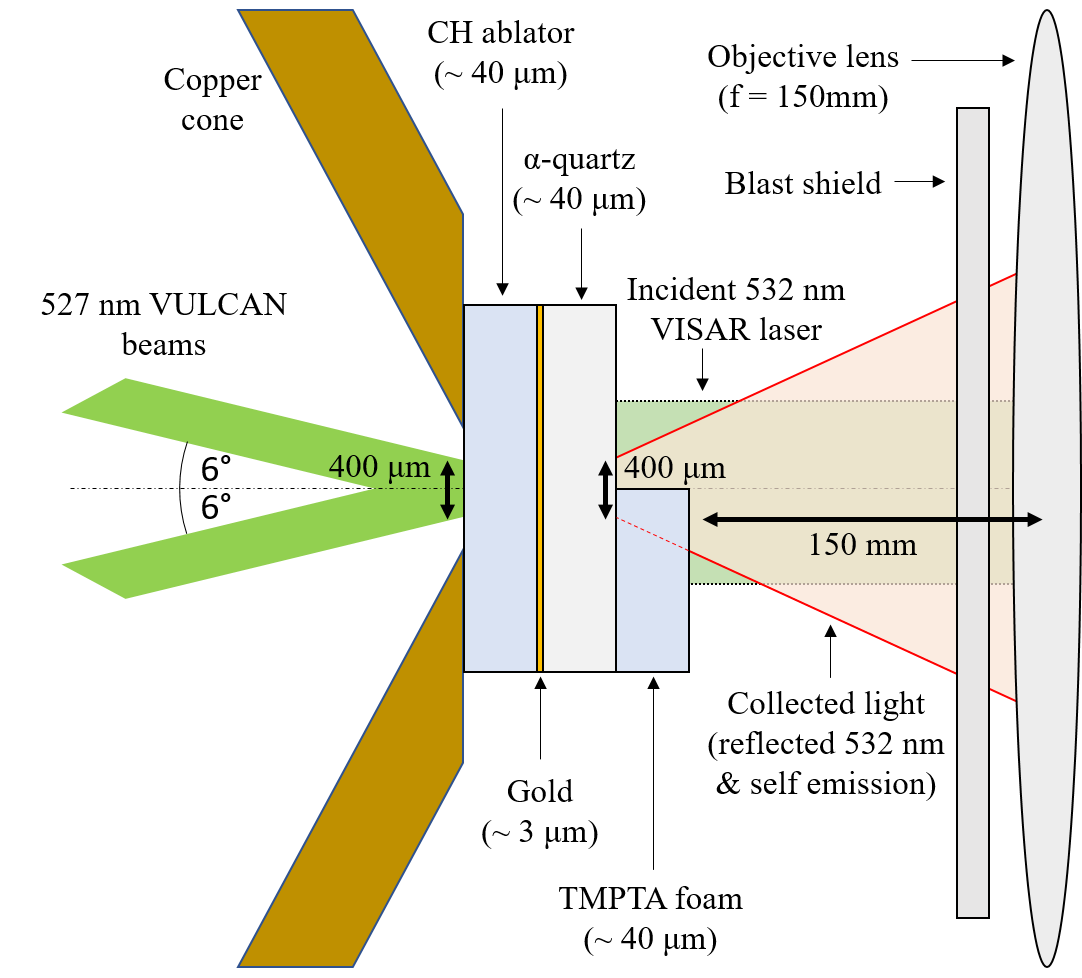
\includegraphics[width=0.45\textwidth]{figures/Experiment/TargetSchematic.png}% Here is how to import EPS art
\caption{\label{fig:target} Simple schematic showing the target and objective lens (top view, not to scale)}
\end{figure}

The shock was roughly uniform over a $\sim$~400~\unit{\micro\meter} diameter. To generate this, the six main VULCAN beams were overlapped spatially to produce a `top-hat' beam with a $\sim$~400~\unit{\micro\meter} diameter. The pulse power profile was also a `top-hat', with a rise and fall time of $\sim$~200~\unit{\pico\second}. 

The target had a step in the rear side, so that the TMPTA foam only covered half of the quartz surface in the $\sim$~400~\unit{\micro\meter} shocked region. This meant that both quartz and foam were visible to the diagnostics, and is similar to targets used in previous experiments to investigate other materials \cite{Falk2014a, Falk2020}. The shock velocity in both layers was measured using VISAR, which was driven using a probe laser reflected off the rear surface of the target. The shock temperature of both layers was determined using streaked optical pyrometry (SOP).

The quartz layer in this experiment was used as a reference material for an impedance matching calculation. The shock velocity in both the quartz and the foam were measured in each shot; this calculation then used this information to calculate the shock state achieved in the foam during that shot. This defines a single point on the foam Hugoniot. By performing a series of shots at different powers (and thus intensities), a number of different points on the Hugoniot were populated.

\subsection{VISAR}

VISAR (or `Velocity Interferometer System For Any Reflector') is a velocity interferometry technique which allows the velocity of a moving surface to be measured. A probe laser is reflected from the measurement surface, and the reflected light captured and passed into the interferometer (often referred to as `the VISAR'). The resulting fringe pattern contains information about velocity changes at the surface. In this experiment, the VISAR is used to determine the shock velocity of both the quartz and the foam.

A simple schematic of a VISAR is shown in figure. The reflected probe laser is split by a beamsplitter, and passes down two seperate legs, before being interfered at a recombination beamsplitter. An etalon is used so that the delay leg has a longer optical path, and thus a longer transmission time. This means that the photons interfering at the beamsplitter from the two different legs entered the interferometer at differnt times, and thus the interference is thus between the laser, and the laser released a short time previously.

The effect of this is that the photons being interfered at the recombination beamsplitter entered the 

This has a significant effect. As there is a difference in the transmission time through the two legs ($\tau$), two photons which arrive at the recombination beamsplitter entered the interferometer at different times. This means the interference is between the laser light, and the laser light a time $\tau$ previously. The resulting interference pattern thus is due to the changes in the phase of the beam over time. 

These phase changes arise from the movement of the target, which is what enables velocity measurements using this technique. Consider the photon that arrives first. To reach the interferometer, the photon travelled from the laser to the measurement surface, and then back to the interferometer - a distance $D$. Now consider the second photon. In the time $\tau$, the surface has moved by a distance $d = \tau u$, where u is the average velocity of the surface over that time. The total distance the second photon travels is therefore $D+2d$ - a longer distance, which results in a phase shift (the factor 2 accounts for the fact that this distance must be covered twice. (A more rigorous analysis would include the fact that it would take some time to cover the distance d, but this is essentially negligible given that the the photon travels at the speed of light).

The total path difference of the two beams at the recombination beamsplitter is therefore $\tau u + \delta$, where $\delta$ is the additional path length introduce by the delay etalon. This path difference results in a phase difference of $\phi = k (tau u + \delta)$, where $k = 2\pi / \Lambda$ is the wave vector. The resulting interference pattern varies according to the phase as $cos(\phi) = cos(k (tau u + \delta)$. As described, and assuming no spatial variation in the reflector, the phase difference would be spatially constant. In order to produce a fringe pattern, the beamsplitter is rotated slightly to introduce a small linear phase ramp in the spatial position $x$, so that $\phi = k (tau u + \delta + xsin\theta)$. This means that the image is now a fringe pattern.

Consider the case where the surface is stationary or moving at a constant velocity, so that $u$ is a constant. In this case, the phase difference $\phi$ between the two signals is constant as a function of time, and thus the interference pattern is stationary - resulting in a static fringe pattern. However, consider the case where the surface velocity is changing, and thus $u$ varies. In this case, the phase will change by $k\tau \Delta u$, and thus the fringe pattern will also move. The pattern will repeat when $k\tau \Delta u = n\pi$ where n is an integer, and thus a full fringe change will occur when the change in velocity $\Delta u = \lambda /2 \tau$.

In this way, the velocity of the surface can be determined. The experiment is begun with a stationary surface, and as the velocity changes the fringe pattern will be altered. The fringe shift F(t) is recorded, and can be converted into a velocity using this `Velocity per fringe', or VPF. This enables dynamic measurement of velocity vs time. The VPF needs an additional correction to account for dispersion, which leads to an actual VPF of \hl{equation}

\subsubsection{Etalon selection}

In order to make the described measurments, the choice of etalons is extremely important. Firstly, the VPF is inversely proportional to the time delay (and thus the thickness) of the etalon. Using a thicker etalon will therefore give a lower velocity per fringe, and thus increased velocity resolution. It is therefore important to choose an etalon that gives appropriate velocity resolution for the velocities likely to be measured to high accuracy.

However, etalon choice also affects the time resolution of the system. The minimum time resolution is set by $\tau$ - if the velocity change occurs in less time than this, it will be recorded as a sudden discontinuity in the phase pattern. If this occurs, then F(t) cannont be known with certainty - the discontinuity could correspond to any integer number of fringes, and the velocity change could thus correspond to any integer number of the VPF.

For rapid changes in velocity, this presents a significant issue. This can be resolved by measuring the same surface with two separate VISARs systems, using two different etalon thicknesses. If the etalons are chosen so that the VPFs are not integer multiples, then the two systems will detect fractional phase jumps of different amounts. As the measured velocity must be the same between the two systems, it is possible to identify which velocity change the discontinuity must correspond to. This experiment used two VISARs for this reason.

\subsubsection{VISAR design}

Most modern VISARs are based on the Mach-Zehnder interferometer design. This has two real advantages. Firstly, both legs travel through a beamsplitter - which means that the beamsplitters introduce no difference in optical path between the two legs. Secondly, using two different beamsplitters for seperation and recombination makes it possible to affect the fringe contrast (and fringe spacing) without impacting alignment.

A labelled diagram of the VISAR used in this experiment is displayed in Figure \ref{fig:Dan_VISAR}. This VISAR was developed and designed by Daniel Eakins. While the main components are the Mach-Zehnder interferometer, the overall device contains a series of optics to aid with alignment.

\begin{figure}
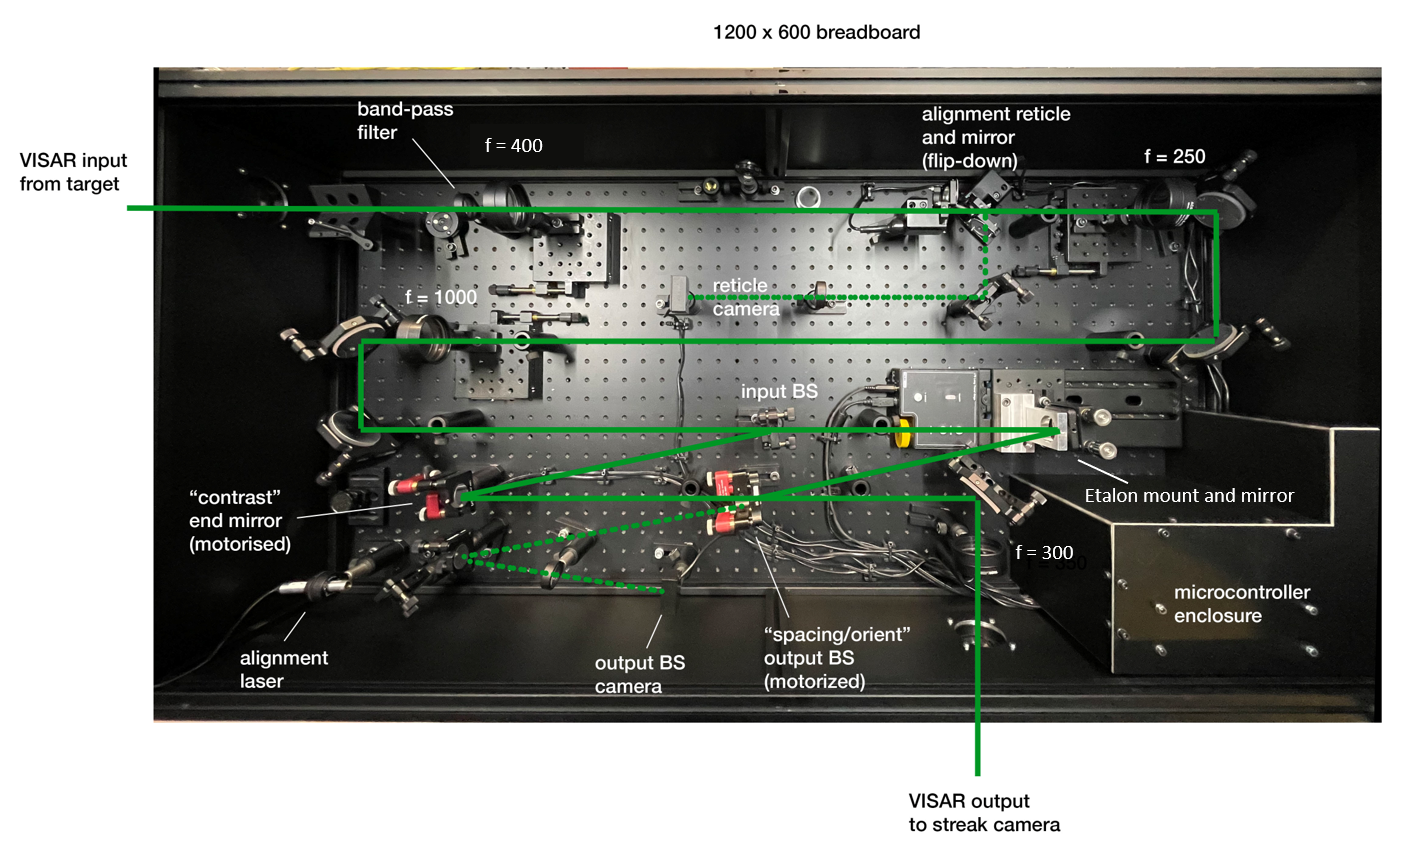
\includegraphics[width=1.0\textwidth]{figures/Experiment/Dan_VISAR.PNG}% Here is how to import EPS art
\caption{\label{fig:Dan_VISAR} The VISAR design used in this experiment (designed and developed by Daniel Eakins). The actual interferometer consists of the components between the input/output beamsplitters, while the other components are used for alignment and to ensure good image contrast. Image provided by Daniel Eakins, with minor changes to labels to reflect the lens setup used in our experiment. }
\end{figure}

The VISAR is internally aligned so that the first flip reticule is positioned in the center of the beampath. This can then easily be used to confirm that the external probe beam entering the VISAR is co-aligned with the system. However, it also serves another important purpose. The etalon and mirror in the delay leg are placed on a piezo-electric motor. As these components are aligned at an angle to the incoming beam, moving them will shift the position of the image. However, it is obviously necessary for the images to be coaligned.

To do this, the etalon is first removed from the delay leg. White light is injected into the VISAR, and the motorised mirror in the delay leg moved until fringes appear. The white light is incoherent, and so this only occurs when the two legs have equal path length - this is sometimes referred to as the `null' or `white-light' position. The system is aligned so that the images are coincident for this seteup, which is confirmed by flipping the reticule into the beam.

The etalon is then inserted. This introduces some refraction of the beam, and thus shifts the image. In order to restore this, the etalon and mirror are moved until the images are colinear again. This offset can be calculated by the formulae \hl{equation}. Ensuring the images are coincident again ensures that the image has good spatial resolution, and also serves to increase fringe contrast - making the signal easier to detect. 

The Mach-Zehnder design of the interferometer has two clear benefits. Firstly, it ensures that both beams pass through one beamsplitter, and thus these components produce no relative path difference between the beams. Secondly, the use of two beamsplitters makes it possible to control the image alignment (and thus contrast) and the linear ramp/fringe spacing independently. The 'contrast mirror' is motorised, and can be adjusted to ensure the best possible overlap between images at the recombination beamsplitter, enabling contrast to be maximised. Independently, the recombination beamsplitter can be rotated to adjust the linear phase ramp, and thus change the spacing of the fringes (this is important, as ensuring adequate fringe spacing is useful for the algorithm to extract fringe motion). 

\subsubsection{Making shock velocity measurements with VISAR}

The previous descriptions describe how VISAR can be used to dynamically measure the velocity of a moving surface. Measuring shock velocity using VISAR introduces additional complexity, as the velocity to be measured is a density interface within the target. To determine what exactly will be measured, it is necessary to consider which surface the VISAR will be reflected from, and it's properties.

The first way to measure shock velocity using VISAR is where the unshocked velocity is transparent to the probe beam, but the shocked material is reflective. In this case, the probe laser can propogate through the unshocked material, and reflect directly off the shock front; this shock front is the measurement surface, and the shock velocity can be measured directly. This is the case for alpha-quartz (the reference used in this experiment), for which the shock front is reflective to 532 nm light for shock pressures above $\sim$ 200GPa.

A different approach is required for opaque materials, such as the foam in this experiment. In this case the probe laser will reflect from the material surface, and so will not reach the shock front - and thus the measurements described so far are not possible. However, the VISAR can be used to detect changes to the surface. Fringes will be produced when the surface is intact, but will suddenly disappear when the surface is blown-out and stops reflecting - as occurs at shock breakout. By using steps in the material of known thickness and using the VISAR to identify the time at which the shock transits the steps, it is possible to calculate the average shock velocity through this region.

\subsubsection{VISAR application in this experiment}

In this experiment, the target has a step structure - so that half the rear surface is exposed quartz, and the other is foam. The spot is positioned over this step - so that half of the VISAR image corresponds to signal from the quartz, and the other half from the foam.

On the quartz side, the probe laser will pass through the quartz and initially reflect from the stationary gold layer. When the shock transits through from the gold to the quartz, the laser will begin to reflect from the shock front instead - leading to a sudden jump from a measured velocity of 0 (the gold surface) to a measured velocity of $U_{s}^{quartz}$. This will be measured dynamically. Eventually the shock will break out of the rear quartz surface, and the fringes will disappear.

The foam is opaque to the probe laser, which continues to reflect off the foam surface - leading to a stationary fringe pattern. This continues until the shock breaks out of this foam surface, at which point the fringe pattern will again disappear.

There are thus two possible measures of the quartz velocity. The average shock velocity can be calculated from the time difference between the shock entering the quartz (i.e. when the signal first changes in magnitude / undergoes fringe motion) and leaving it (when the fringes disappear). The quartz velocity as a function of time can also be determined from analysis of the fringe pattern between these times. The average foam shock velocity can be calculated using the time between shock breakout in the quartz (which coincides with shock entry into the foam), and the foam fringes disappearing.

\subsubsection{VISAR analysis}

A toy model is presented which simulates how such VISAR data would look, for two separate etalons. The timings and quartz shock velocity is determined from pre-shot hydrodynamic simulations, and used to generate the corresponding fringe pattern. This in turn has been analysed, according to the analysis procedure described in the appendix, to reproduce the measured velocity plot.





%It is also necessary to include a translation offset in the delay leg, to account for the refractive index of the etalon. The etalon is placed at an angle to the beam, to avoid reflections from the etalon surfaces introducing interference; this however introduces refraction, which would shift the position of the beam at the recombination beamsplitter. To avoid this, the etalon and mirror in the delay leg are placed on a motorised stage. The etalon is removed, and the mirror translated to find the position corresponding to zero path difference. The etalon is then reinserted, and the mirror/etalon then repositioned until the image is coincident with the null position. this distance, $d = h(1 - 1/n)$ is then recorded. 

%The optical path difference between the delay and non-delay legs is $2(hn - h)$ (as the h thickness of etalon, with optical path $hn$, replaces a distance $h$ of air with a refractive index of 1. The factor 2 comes from the fact that the light passes through this etalon twice). Combining this and the translation offset gives a total path difference of $2h(n - 1/n)$, and thus an optical time delay of $\tau = 2h/c (n - 1/n)$.

%In any interferometer, the fringe frequency is the frequency difference (or beat frequency) of the two legs. In the velocity interferometer, this frequency difference is determined by the time dependent Doppler shift of the reflected light. The light being interfered is a reflection from the measurement surface at a time t1 and a time t1 + $\tau$. The Doppler shift of the reflected beam is dependent on the surface velocity, and thus the frequency difference between these two signals is also linked to the velocity. It is thus clear that the beat frequency will change as a function the velocity of the measurement surface, and thus the fringe pattern will change. However, the operation of the VISAR can be better illustrated by considering the path difference experienced by photons.

%The effect of the VISAR is to interfere photons that were reflected from the measurement surface at different times. At any given time, the photons being interfered at the recombination beamsplitter passed through the seperation beamsplitter at a time $\tau$ apart, and thus reflected from the measurement surface at different times. The measurement surface has a velocity $v(t)$, and thus a position $x(t)$. There will therefore be an additional path difference $\delta x$ between the two paths from the movement of the surface, introducing an additional optical time delay of $2h/c \delta x$.

%If the surface is stationary, then $\delta x$ is constant (zero) and the phase difference between the two legs is constant. The resulting interference pattern is thus unchanging as a function of time. If the surface is moving at a constant velocity, then $\delta x$ is also constant as a function of time. However, if there velocity of the surface is changing, then the phase change will also change, and the fringe pattern will move to reflect this. If the change is large and occurs much faster than the time resolution of the detector, this will result in discontinuities in the fringe pattern.

%The phase difference associated with this delay is given by $\Deltat\phi = kx = x/\Lambda$. As the fringe pattern is given by sin($\Deltat\phi$), one complete fringe corresponds to a phase difference of 2 pi.

\subsection{Streaked Optical Pyrometery} \label{SOP theory}

Streaked Optical Pyrometry enables the temperature of a body to be determined, based on it's thermal emission \cite{Zeldovich1966}. Emmitted light from the target is captured using measurement optics. This light is broadband, but can be filtered down to a narrow wavelength range using appropriate filters. This filtered emission is then recorded on a streak camera, which records the intensity vs time vs a spatial dimension.

%As described in \cite{Miller2007}, the intensity recorded on a streak camera at a given pixel is given by 
%\begin{equation} I = \frac{\Delta t}{G} \int {\Phi_S(\lambda) T_x(\lambda)SR(\lambda) d\lambda}, \end{equation} where $\Delta t$ is the dwell time (the amount of time over which signal is acquired for a given pixel), $G$ is the streak camera gain between photoelectrons and analogue to digital units, $T_x(\lambda)$ is the transmission between the object and the camera, and $SR(\lambda)$ is the SOP response function. $\Phi_S(\lambda)$ is the radiant power from the source. The power from the source that maps to a given pixel can be calculated as 
%\begin{equation} \Phi_S(\lambda) =  \int_{A_{pixel}}{ dA} \int_{\Omega_{lens}} { L_S(\lambda) d\Omega}, \end{equation}
%where $A_{pixel}$ is the source area represented per pixel, and $\Omega_{lens}$ is the solid angle captured by the imaging system. $L_S{\lamba}$ is the spectral radiance of the source. For a given optical setup of the streak camera (i.e. where the target is placed at the same location, the imaging system is not being changed, and the streak camera settings are constant), then these equations can be combined and simplified to 
%\begin{equation} I = \alpha \int {L_S(\lambda) T_x(\lambda)SR(\lambda) d\lambda}, \end{equation} where the proportionality constant $\alpha$ contains a number of variables relating to the specific setup used.

Following the derivation given in \cite{Miller2007}, the intensity recorded on a streak camera at a given pixel is given by \begin{equation} I = \int {\Delta t} dt \int {\Phi_S(\lambda) T_x(\lambda)SR(\lambda) d\lambda}, \end{equation} where $\Delta t$ is the dwell time (the amount of time over which signal is acquired for a given pixel), $T_x(\lambda)$ is the transmission between the object and the camera, and $SR(\lambda)$ is the SOP response function. $\Phi_S(\lambda)$ is the radiant power from the source. The power from the source that maps to a given pixel can be calculated as 
\begin{equation} \Phi_S(\lambda) =  \int_{A_{pixel}}{ dA} \int_{\Omega_{lens}} { L_S(\lambda) d\Omega}, \end{equation}
where $A_{pixel}$ is the source area represented per pixel, and $\Omega_{lens}$ is the solid angle captured by the imaging system. $L_S{\lamba}$ is the spectral radiance of the source. For a given optical setup of the streak camera (i.e. where the target is placed at the same location, the imaging system is not being changed, and the streak camera settings are constant), then these equations can be combined and simplified to 
\begin{equation} I = \frac{B \Deltax W_s \Omega_{lens}}{\eta M^2} \int {L_S(\lambda) T_x(\lambda)SR(\lambda) d\lambda}, \end{equation} where the variables outside the integral all relate to the specifics of the optical setup and streak camera settings ($B$ is the CCD binning, $W_s$ is the slit width, $\eta$ is the sweep rate, and $M$ is the magnification).

The source is then assumed to emit as a black body, such that the spectral radiance can be calculated using Planck's law, 
\begin{equation} L_S(\lambda) =  \frac{2hc^2}{\lambda^5} \frac{1}{[\exp(\frac{hc}{\lambda T}) - 1]}, \end{equation} where $T$ is the black-body temperature. The SOP signal is therefore given by 
\begin{equation} I = \frac{B \Deltax W_s \Omega_{lens}}{\eta M^2} \int {\frac{2hc^2}{\lambda^5} \frac{<T_x(\lambda)SR(\lambda)>}{[\exp(\frac{hc}{\lambda T}) - 1]} d\lambda} \end{equation}
The incoming light is filtered down to a narrow wavelength band. Is is thus approximated that the fourier spectrum of the incoming light can be approximated as a delta function, at the central wavelength of this band. This simplifies the SOP signal to
\begin{equation} I = \frac{B \Deltax W_s \Omega_{lens}}{\eta M^2} \frac{2hc^2}{\lambda_0^5} \frac{T_x SR }{ [\exp(\frac{hc}{\lambda T}) - 1]} , \end{equation}
This equation can then be rearranged to give an expression for temperature in terms of the measured intensity, 
\begin{equation} T = \frac{T_0}{\ln(1 + \frac{A}{I})}, \end{equation}
where $T_0 = \frac{hc}{\lambda_0}$ is a constant, and $A$ is a calibration constant,
\begin{equation} A = \frac{B \Deltax W_s \Omega_{lens} 2hc^2 <T_x SR>}{\eta M^2 \lambda_0^5} , \end{equation}
which is constant for a constant experimental setup and streak camera settings\footnote{I need to decide where/how to include gain in this derivation}.

Real samples do not emit as perfect black-bodies. This can be accounted for by factoring in the emissivity of the body, which can be calculated as $\eta = 1 - R$, where $R$ is the reflectivity (from Kirchoff's second law, stating that absorption and emissivity are equal for an object in thermal equilibrium). To account for this in the above derivation, the SOP streak intensity $I$ in replaced in every instance by $I/(1-R)$. This results in an equation for the grey-body temperature of the sample of \begin{equation} T = \frac{T_0}{\ln(1 + \frac{(1-R)A}{I})}. \label{eqn: SOP eqn} \end{equation}

The SOP diagnostic can be absolutely calibrated for a fixed setup, where the components are not regularly changed. This process is outlined for the Omega setup in \cite{Gregor2016}; by making measurements over a series of wavelengths using an absolutely calibrated light source, the different wavelength dependent functions (such as spectral response and transmission) of the camera can be determined. The value of $A$ can then be calculated with confidence for different wavelengths and different camera settings. 

\subsubsection{SOP in this experiment}

In this experiment, SOP was used to measure the signal from both the quartz and foam. However, as the SOP was built from scratch during the experimental run there was not sufficient time nor equipment for an absolute calibration to be performed. Instead, the quartz was used as a known temperature reference, and calibration was performed on-shot.

To do this, the expected quartz shock temperature is required. This was estimated from the VISAR-measured shock velocity using a power law fit from \cite{Millot2015}, \begin{equation} T(K) = 1421.9 + 4.3185 U_S^{2.9768} \label{eqn:Temp fit} \end{equation}, determined from the experimental data in \cite{Hicks2006}. The corresponding SOP intensity signal could thus be used to calculate the on-shot calibration constant $A$ in equation \ref{eqn: SOP eqn}. With $A$ for the shot determined, the foam SOP intensity could therefore be used to calculate the foam temperature. This on-shot calibration leads to large uncertainty, as error in the shock velocity measurement and the above model both affect the calculated foam temperature.

\subsection{X-ray pinhole camera}
An X-ray pinhole camera imaged the front surface of the target. As the VULCAN beam irradiated the ablator and target, high energy X-rays are emitted in all directions. The X-ray pinhole camera consists of a small aperture seperated from x-ray sensitive film by a known distance L. The film is shielded so that only x-rays passing through the aperture can reach the screen. This results in a magnification $M$ equal to the ratio $M = L/D$, where D is the distance from the target to the aperture. After each shot, the image plate is scanned to give a two-dimensional image showing the x-ray energy received. The minimum energy of the detected X-rays can be set by placing a filter (a thin film of aluminium) over the aperture.

\begin{figure}
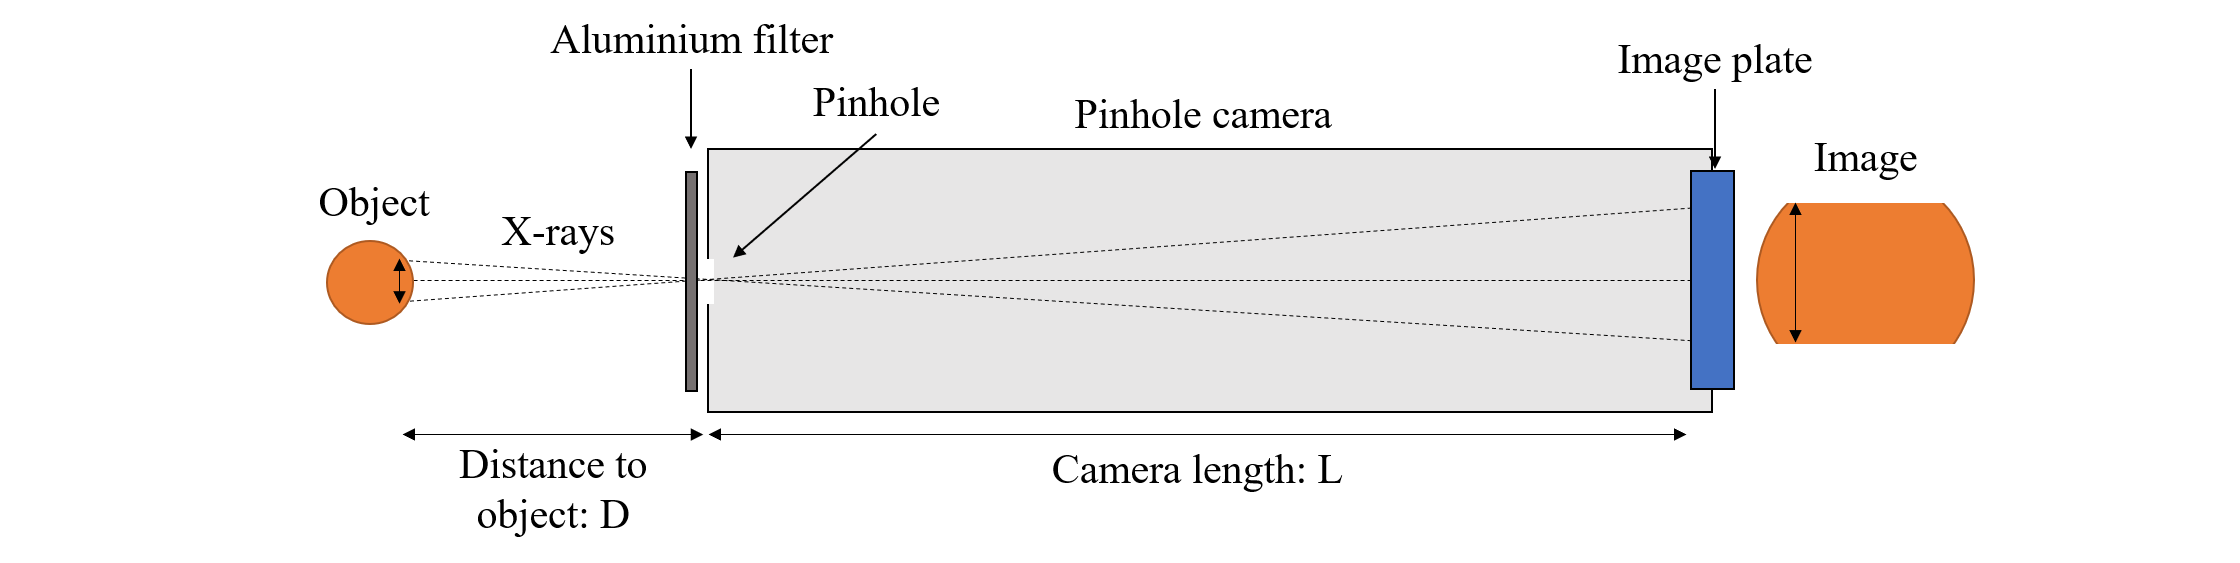
\includegraphics[width=1.0\textwidth]{figures/Experiment/PinholeSchematic2.png}% Here is how to import EPS art
\caption{\label{fig:Pinhole schematic} A schematic of a pinhole camera. The distance D between the object and the camera sets the field of view and the magnification.  }
\end{figure}

It is possible to quantify the amount of X-rays received by the image plate, but such an analysis was not necessary/useful for this experiment. Instead, the camera was used to indicate the spatial characteristics of the VULCAN spot. This was useful for confirming where the laser spot hit on the target, that there was a good overlap between the six beams, and to estimate the spot size.

\subsection{Fiducial} \label{Fidu theory}
A fiducial was setup on one of the VISAR streak cameras. A fibre-optic cable was setup behind one of the mirrors in the VULCAN laser chain. These mirrors were slightly lossy, and the fibre `picked-off' some of this parasitic signal. The other end of the fibre was positioned so that it produced a small dot on the side of one of the VISAR streak cameras. The fibre length was such that this parisitic VULCAN signal reached the streak camera in the same streak window that the main signal from the target was detected. Images of this setup can be seen in the appendix.

Two-minute shots (low-power VULCAN shots, so-named as they can be fired every two minutes) were performed without a target present, so that the VULCAN pulse could be measured directly on the streak camera. By doing so, the time delay between the VULCAN shot reaching the target and the fiducial signal showing on the streak could be determined. This meant on subsequent full power shots, where the VULCAN pulse could not be seen directly due to the presence of the target, it was possible to calculate the time at which the pulse was applied based on the fiducial signal.

\subsection{Calorimetry}
Calorimeters, which returned a voltage signal based on the fluence of light received, were in place behind a leaky mirror in each of the six beams. These were calibrated to provide an estimate of the energy in each beam for each pulse (one of these was partly blocked by the fiducial, and so returned a low signal - as the six beams were delivering similar energies, an average of the other beam energies was used for this beam when estimating the total pulse energy).

The VULCAN beam is generated at IR, and had to pass through a frequency-doubling crystal to be converted to 527 \hl{\nano\meter}. The facility staff performed a series of calibration shots. On these shots, larger calorimeters were set up in the main beam path to measure the full energy in each beam, while the orientation of the crystal was optimised. This also allowed for calibration of the smaller, on-shot calorimeters; the voltage the parasitic calorimeters measured as a function of the energy measured by the full calorimeters were recorded, and used to find the relationship between voltage and energy, so that the energy of the beam on shot could be calculated.

\subsection{Pulse length}
Photodiodes were placed behind the final set of mirrors in the Vulcan chain (a different set of mirrors to the calorimeters). Images of this setup can be seen in the appendix. These measured the pulse shape of each beam on every shot, and saved it to an oscilloscope - allowing the pulse length and temporal shape of each beam to be observed.

\section{Preparation for the experiment}

\subsection{Development of the optical setup}

An optical setup was required to collect and transmit the self-emitted light to the SOP. Further optics would also be required to transmit the probe laser to the rear of the target, and to collect the reflected beam and deliver it to the VISAR. 

Both VISAR and SOP were operated normal to the rear target surface. While it is possible to operate VISAR off-axis, this has not previously been done in experiments at these intensities (and would also require a correction to the data). Operating both diagnostics in this configuration meant that a shared optical system would be required to transmit the light from the target to the diagnostics, with a dichroic mirror used to separate the 532 nm light from the self-emission. Similar setups are used on Omega \cite{Miller2007, Gregor2016}.

This optical system had to minimise transmission losses to ensure a strong signal at the diagnostics. In particular, there was a risk that the self-emission could be relatively weak - and thus it was desirable to avoid placing any beam-splitters in the shared optical relay. This meant that the probe laser injection would need to occur prior to the dichroic mirror, resulting in the basic experiment design displayed in Figure \ref{fig:Simple experiment schematic}.

\begin{figure}
  \centering
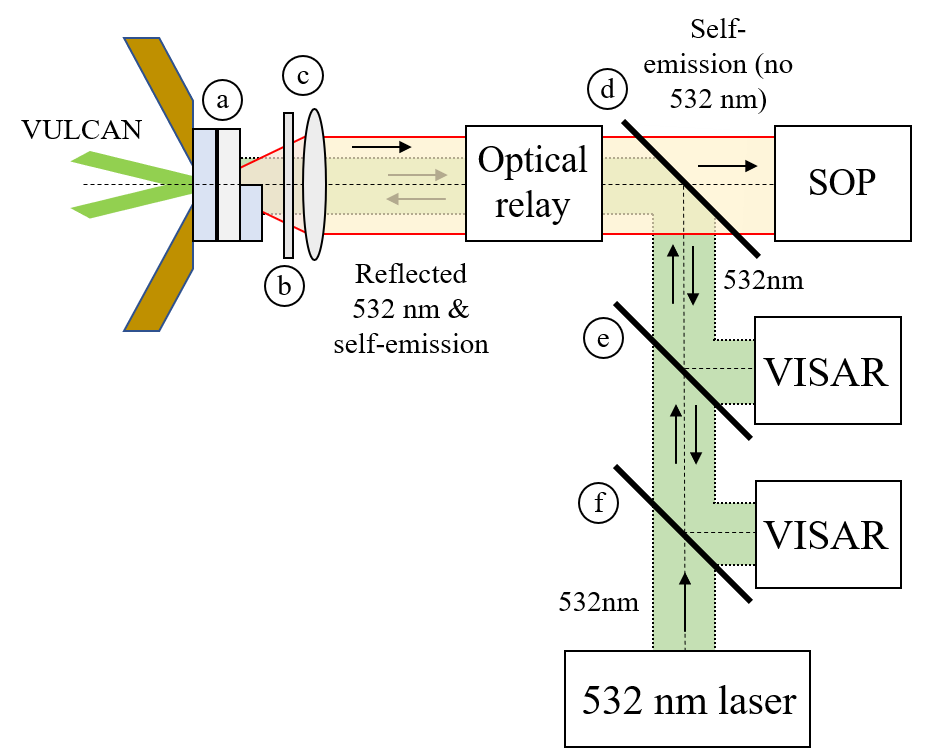
\includegraphics[width=0.8\textwidth]{figures/Experiment/Simple experiment schematic.png}% Here is how to import EPS art
\caption{\label{fig:Simple experiment schematic} A simple schematic of the initially proposed experimental layout. Reflected 532 nm light from a probe laser, and the self-emission, are captured from the target (a) by an objective lens (c) protected by a blast shield (b). This captured light passes through an optical relay, which magnifies it and transports it to the diagnostics. A dichroic mirror (d) reflects the 532 nm light out from the broadband light. This reflected 532 nm light is split and sent to the two VISAR diagnostics via two beamsplitters (e and f). The remaining broadband light passes through the dichroic mirror to the streaked optical pyrometer. The 532 nm laser is injected through the back of the second VISAR beamsplitter, and travels through the full optical relay to illuminate the target. This setup avoids the need for the self-emission to pass through a beamsplitter on it's route from the target to the SOP.  }
\end{figure}

A number of factors needed to be considered in the design of this system:

\begin{itemize}
    \item \textbf{Optical relay spacing}: The spatial configuration of the target chamber and area set limits on the optical relay design. Injecting the probe laser through the VISAR beamsplitter required the laser to be located relatively close to the diagnostics (to avoid a long beam path around the target area). This set constraints on the positions of the optical benches in the target area, and meant that it would be necessary for the optical relay to transmit the light through the south chamber window (which was furthest from the target position). This window was 1.5m away from the target position, with a further 1.3m of window/free space propagation before the optical table would be reached.
    
  \begin{figure}
  \centering
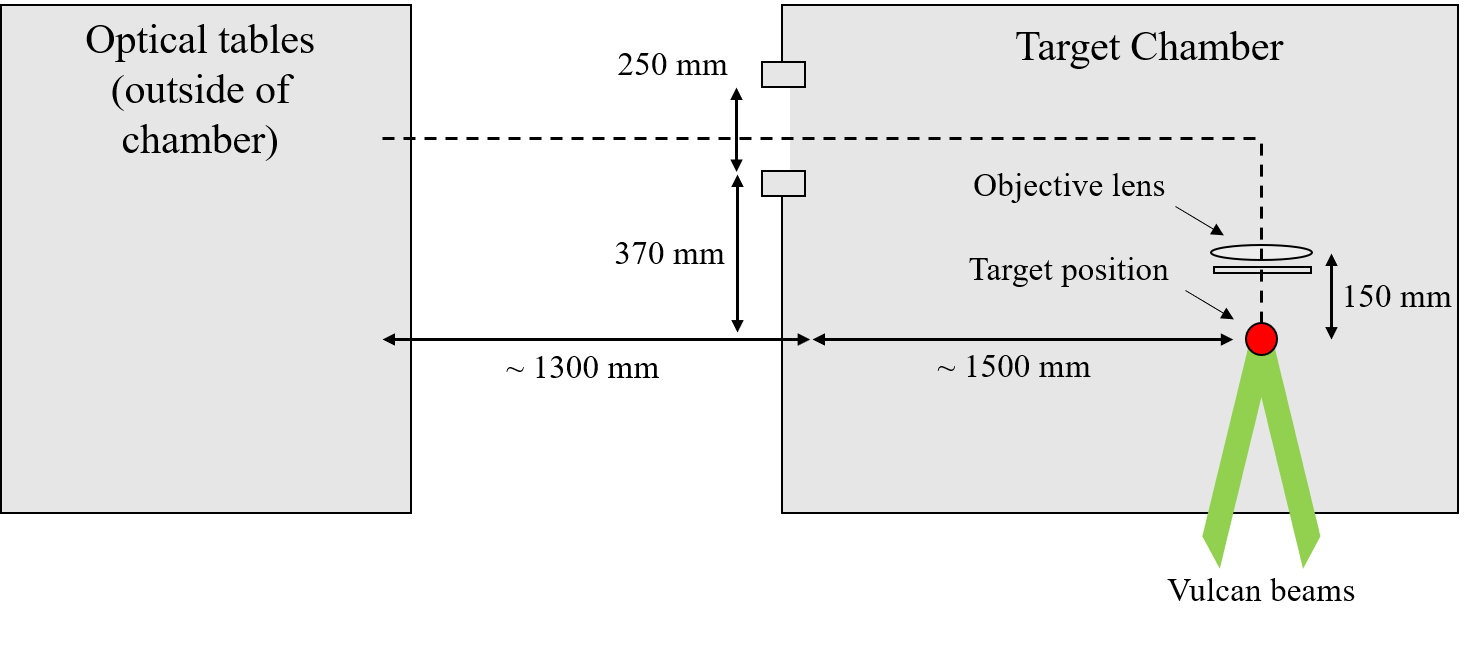
\includegraphics[width=0.8\textwidth]{figures/Experiment/Experiment Spacing.png}% Here is how to import EPS art
\caption{\label{fig:Experiment} A simple schematic (not to scale) showing the spacial considerations for the optical relay. There was a useable distance of optical table of $\sim$ 1500 mm of optical table within the chamber before the window. There was then a further $\sim$ 1300 mm gap (in which no lenses could be placed) before the main optical tables.  }
\end{figure}  
    
    \item \textbf{Magnification}: The SOP had a slit width of 4.46 \unit{\milli\meter}, while the VISAR had a width of 17.4 \unit{\milli\meter}. The imaged area was 400\unit{\micro\meter} in diameter, and should be magnified to fill as much of this area as possible. The VISAR already had a number of built in lenses (of which only the first could be changed), and so it was necessary to design a system which would provide appropriate magnification for both diagnostics as well as transmitting the beams with minimum losses over the relevant distances.
    
    \item\textbf{Components}: The optical components required for the relay and for the diagnostic systems also needed to be identified and purchased. This included: a dichroic mirror, low-pass and high-pass filters for the SOP, and notch filters (to prevent any 527nm Vulcan noise affecting the VISAR signal). Many of these components, as well as the optical components within the VISAR, were only available in 1-inch versions - which set limits on the beamsize.
    
    \item \textbf{Diagnostic positioning}: Finally, it was necessary to consider how the diagnostics and beam paths would actually fit on the optical table. The VISARs in particular were large pre-assembled systems with fixed entry points for the beam path. The 1-inch optical components meant it was necessary to minimise the distances between the VISARs and the final lens in the optical relay to avoid transmission losses, but this was challenging to achieve practically.
    
\end{itemize}

To assist with this design work, a Matlab script was produced to perform ray-tracing (using simple geometrical optics) of light through a lens system. This allowed the expected losses through a given system to be estimated. A number of setups were explored to find a system which minimised losses while being compatible with the above considerations. The final design achieved this, with no expected losses (as predicted by this simple approximation). 

Figure \ref{fig:Full experiment schematic} shows a full schematic of the experiment. The optical relay consists of 5 lenses (L1 to L5). The dichroic mirror then takes the collimated beam, and sends the signal to the SOP/VISARs. The SOP consists of a 400 nm long pass filter and 500 nm short pass filter, leaving only 400 - 500 nm wavelengths, before a final lens S1 focusses the beam on to the streak camera. Beamsplitters send the VISAR beam into the VISAR system (the 'VISAR' here is used to refer to the full system shown in Figure \ref{fig:Dan_VISAR}, rather than just the interferometer). The beam passes through a notch filter, followed by the 4 lenses within the VISARs (and the interferometer, which is not shown), before being focussed onto the beam splitter by lens V5 (and further focussed in the vertical direction by the cylindrical lens V6). The lens spacing can be seen on the CAD models in the appendix. The spacing between focussing pairs is fixed by the focal distances of the lenses. There was some flexibility in the spacing between L1 \& L2 and L3 \& L4; however, the distance between L5 \& V1 for each VISAR had to be kept below 1m to avoid losses (otherwise the beam would be too large for the 1 inch components inside the VISAR), and the distance from V4 to the VISAR streak camera also needed to be under 1m. The filters short pass filter (c) was also a 1 inch component, and so it was important to place this close to the dichroic mirror.

\begin{figure}
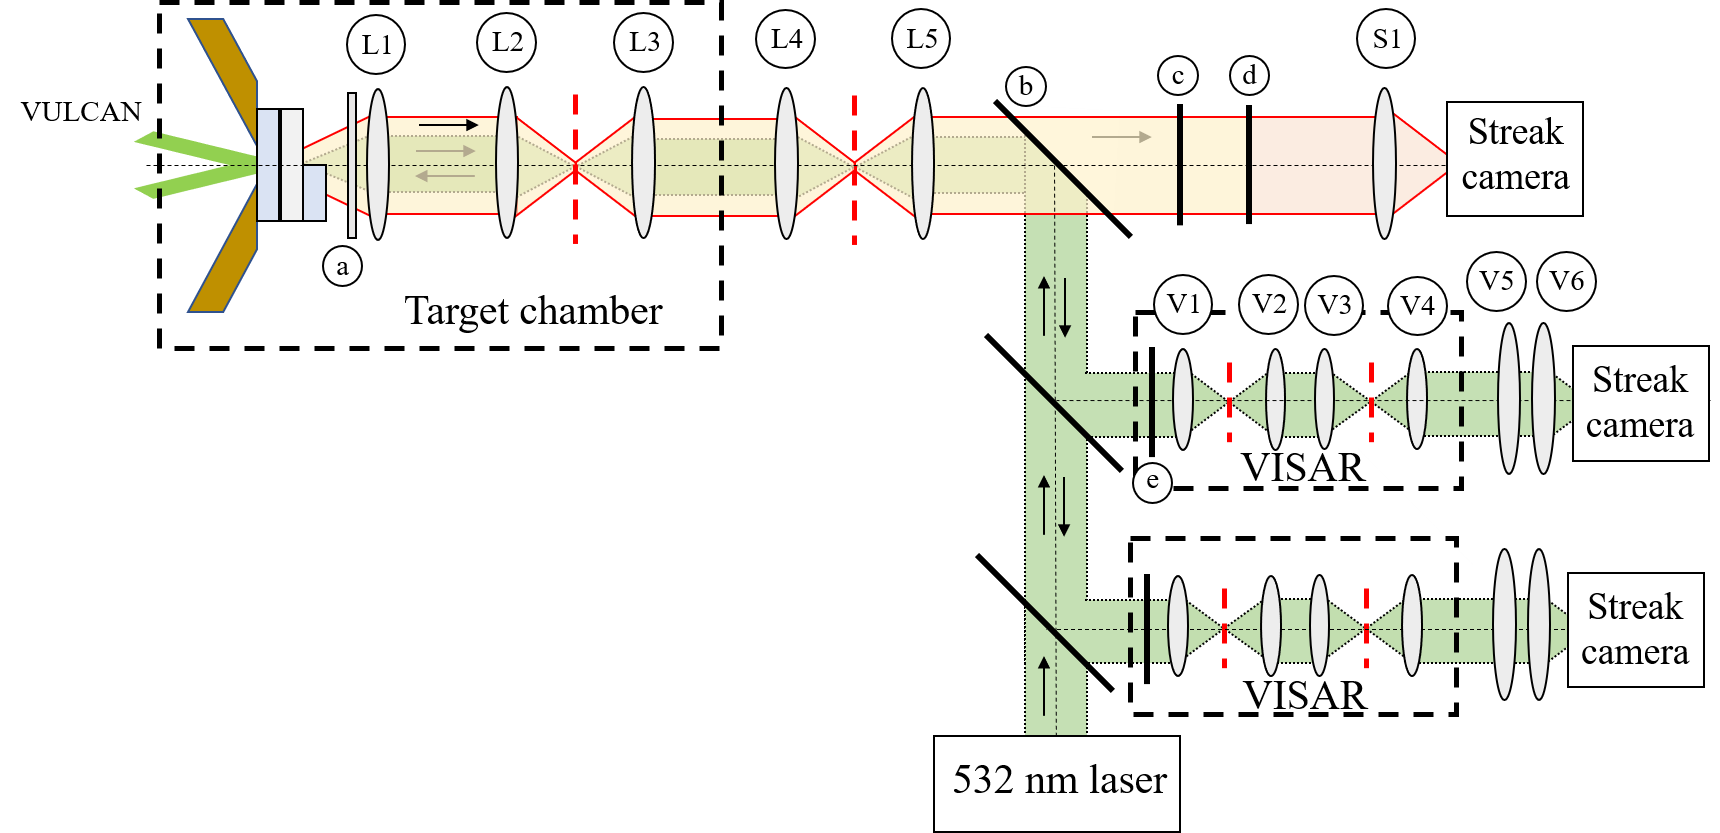
\includegraphics[width=1.0\textwidth]{figures/Experiment/Full experiment schematic.png}% Here is how to import EPS art
\caption{\label{fig:Full experiment schematic} The full proposed schematic. Lenses labelled 'L' form the optical relay, while those labelled 'S' are part of the SOP and 'V' are part of the VISAR. The two VISARs are identical in terms of components. The dashed red lines represent the positions of image planes. The interferometer in the VISAR is not pictured (it can be viewed in Figure \ref{fig:Dan_VISAR}), but is positioned so that the second beamsplitter is positioned at the second image plane. The focal lengths are as follows: L1 = 150mm, L2 = 700mm, L3 = 500mm, L4 = 700mm, L5 = 250mm, S1 = 300mm, V1 = 400mm, V2 = 250mm, V3 = 1000mm, V4 = 300mm, V5 = 300mm, V6 = 200mm (cylindrical). Also indicated are the other components in the beamline: a blast shield to protect the objective lens (a), the dichroic mirror (b), the short-pass (c) and long-pass filters (d) for the SOP, and notch filters (e) for the VISARs.}
\end{figure}

Figure \label{fig:Original CAD} shows a CAD model (produced by the CLF CAD team) of the real setup used in the experiment, which satisfied all these spatial requirements. The measurements are provided in the appendix. Figure \ref{fig:Ray trace} then shows the output of the ray tracing script for the target to SOP and target to the second (furthest VISAR). It can be seen that none of the rays are lost from the lens setup, and thus that 100\% of the light captured by the objective lens is transmitted to the streak cameras.

\begin{figure}
\includegraphics[width=1.0\textwidth]{figures/Experiment/OriginalCAD.png}% Here is how to import EPS art
\caption{\label{fig:Original CAD} A to scale CAD model of this setup as used in the experiment. All spatial criteria are met.}
\end{figure}


\begin{figure}
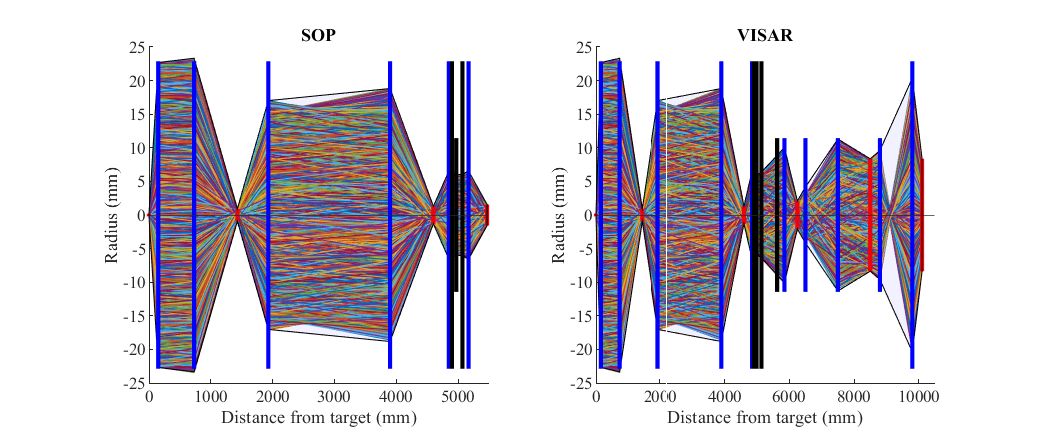
\includegraphics[width=1.0\textwidth]{figures/Experiment/RayTracing.eps}% Here is how to import EPS art
\caption{\label{fig:Ray trace} Ray tracing simulations through the full lens systems for the SOP and VISAR. The components are placed with the real experimental spacing. Lenses are represented by blue lines, while other components (dichroic mirror, beamsplitters, filters) are represented by black lines. Rays are generated at a number of equally spaced point on the target, over angles ranging from 0 to 180 degrees relative to the vertical. These rays are propagated through the system according to simple geometric optics through thin lenses. At each component position, the radial position of each beam is compared to the component size; if it is bigger, the ray is considered 'lost'. This approach suggests transmission through the system greater than 95\% for both the VISARs and SOP.}
\end{figure}

\subsection{Target design and hydrodynamic simulations}

\subsubsection{Layer choice and thickness}

The initially proposed target was based on multi-layer step target desgins successfully used in previous experiments \cite{Falk2014a, Falk2020}. The initial proposal used an aluminium layer as the reference, but this was replaced with quartz so that the velocity of the shock could be measured directly using the VISAR \footnote{The original proposal had suggested that the VISAR could be used to measure the free surface velocity of the aluminium and foam. Under this approach, the VISAR reflects from the rear of an opaque target. The target is shocked, and the shockwave reaches the rear surface, which undergoes free surface expansion. The free surface velocity is measured by the VISAR; this is generally approximated as being twice the particle velocity within the shocked medium. This is a common approach at lower pressures, but it is not possible in this regime - as the shocked material becomes a plasma, the rear surface is destroyed and thus the free surface velocity cannot be measured. As such, the target design was changed to replace the aluminium with quartz, and the foam shock velocity was instead determined from the transit time}. The four layers and step structure led to a relatively complicated target.

The thicknesses of the different layers were influenced by a number of factors. These are listed below:

\begin{itemize}
    \item \textbf{VULCAN pulse length/energy capabilities}: In order to ensure a sustained shock, it was intended that the laser pulse should last until the shock broke out from the rear of the target. There was an upper limit on how long VULCAN could sustain a pulse for (particularly at high intensity, where high energy is required), and this therefore prevented very thick targets with long shock propagation times.
    \item \textbf{Secondary shocks}: Hydrodynamic simulations showed that when the shock crossed from the gold layer into the quartz, a release wave would propagate back through the target. Upon reaching the ablation front, this would generate a second shock which would travel through the target. Depending on intensity/target thickness, this secondary shock could catch up and merge with the primary shock. This would mean the shock strength would change, which would prohibit the use of the impedance matching calculation. This effect was heavily influenced by the thickness of the different layers, and needed to be avoided. An example of this behaviour can be seen in FIGURE.
    \item \textbf{Fabrication constraints}: Target fabrication indicated that the 40~\unit{\micro\meter} was the minimum thickness of quartz/foam that they would be able to produce.
    \item \textbf{Preheating}: The gold layer would need to be sufficiently thick to prevent preheating of the quartz/foam. 
    \item \textbf{Avoiding direct laser heating of gold}: The ablator needed to be sufficiently thick so that the ablation front remained in this layer throughout the laser pulse, and thus the gold did not undergo direct laser heating.
\end{itemize}

Hydrodynamic simulations were performed to find the optimal target design. The minimum 40~\unit{\micro\meter} thickness for the quartz and foam was chosen to mitigate the pulse length concerns. This also was required for the second shock; the thicker the quartz/foam layers were, the more distance there was for the second shock to catch the primary shock in. 40~\unit{\micro\meter} quartz/foam thickness the second shock was already a significant problem. 

Increasing the gold and ablator thicknesses were both found to delay the second shock, improving this issue (the gold/quartz interface was moved further from the ablation front, which meant the second shock (which has to travel this distance twice once it is generated at this interface) had a longer distance to travel relative to the first). Simulations were performed investigating the potential gold/ablator thicknesses that could be used, and the impact this would have on the required laser pulse time/energy at different intensities.

The selected design used a 40~\unit{\micro\meter} ablator, and a 3~\unit{\micro\meter} gold layer. In Hyades, this led to the required pulse times/pulse energies as a function of intensity seen in Figure \ref{fig:VULCAN energy} - remaining under the 600 J maximum energy of VULCAN for the full planned intensity range \footnote{In spherical hydrodynamic simulations a multiplier is applied to the incoming laser energy to account for losses such as cross-beam energy transfer. CBET is likely to be less important for this setup, but there likely would be some loss. The simulations presented in this section do not include such a multiplier, and so it's likely that the shots would require a larger energy/pulse time for a given intensity. However, as the highest intensity in Figure \ref{fig:VULCAN energy} requires only 500 J as opposed to the 600 J VULCAN can deliver, there is some additional energy available to account for this. }. The target did not experience second shock merger over this intensity range. The simulations also suggested that the ablation front remained in the ablator for all of these intensities, and that the 3\unit{\micro\meter} gold layer would prevent preheating of the foam to less than 10K. Hydrodynamic simulations cannot be expected to describe preheating with high accuracy, as they do not include many of the laser plasma effects; however, previous experiments have used similar gold thicknesses, and did not report substantial amounts of preheat - suggesting that this thickness would be appropriate.


\begin{figure}[hbt!]
\centering
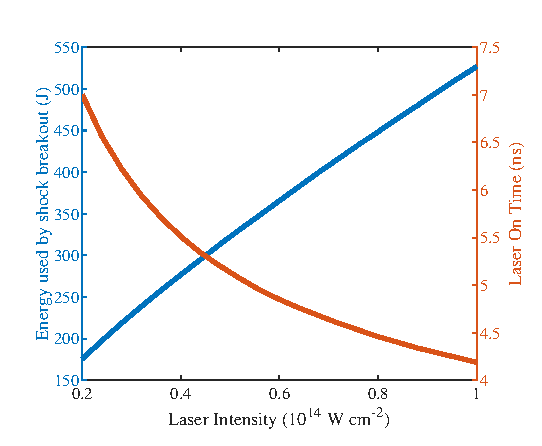
\includegraphics[width=0.8\textwidth]{figures/Experiment/EnergyandPulsetimes.eps}% Here is how to import EPS art
\caption{\label{fig:VULCAN energy} The required VULCAN pulse times as a function of intensity, if the pulse is to be applied until shock breakout from the rear of the target, as simulated in HYADES. The shock breakout time is identified from simulation at each intensity, which defines the required pulse time. The energy of this pulse (given the known intensity and required pulse time) can also then be calculated. There is an inverse relationship between these two parameters; higher intensities result in faster shocks (and thus shorter required pulse lengths), but the increased intensity also means that the required energy of the pulse is higher (i.e. the pulse length does not reduce by enough to balance the increased power).}
\end{figure}

\subsubsection{Additional considerations}

There were also a number of practical concerns with the target assembly. Firstly, it was key to the experiment that no glue layers were used in the target, for a number of reasons. Firstly, there was concern that glue might wick into the foam, which would change it's behaviour. Secondly, a glue layer between the quartz and the foam would prevent impedance matching being performed, as these two materials would not be in contact. Finally, a glue layer between the gold and the quartz would make it difficult to determine when the shock entered the quartz from the glue layer. This meant that the target had to be constructed without glue. The manufacture of the targets was handled by CLF target fabrication (particularly Chris Spindloe, Sam Irving, David Haddock, and Donna Wyatt). The ablator and gold coatings were grown directly on to the quartz, so that no glue was required here. The foam was placed in position on the quartz, so that one foam edge was centered on the quartz piece (giving the step structure). The foam was then 'tacked' to the quartz with glue at the corners - this was sufficiently far from the center of the target that there would be no glue between the layers in the shocked/imaged region.

Secondly, coatings were required for the quartz. An anti-reflection coating was requested on the quartz surfaces, to prevent spurious reflections and 'ghost fringes' (where persistent fringes are seen in the VISAR data from the interference between light reflecting from different surfaces in the material).

\subsection{Hydrodynamic simulations}

The hydrodynamic simulations mentioned in the previous section also enabled the expected conditions in the quartz/foam to be investigated. A selection of the key shock variables can be seen in Figure \ref{fig:PreExpHydro}. These simulations were performed in Hyades and were used to inform etalon selection, as well as confirming that the quartz pressure was sufficient for a reflective shock front. Experimental collaborators also ran simulations of this in Multi, Helios, and FLASH, and good agreement was observed (a comparison between these codes can be seen for the post-experiment simulations).

\begin{figure}[hbt!]
\centering
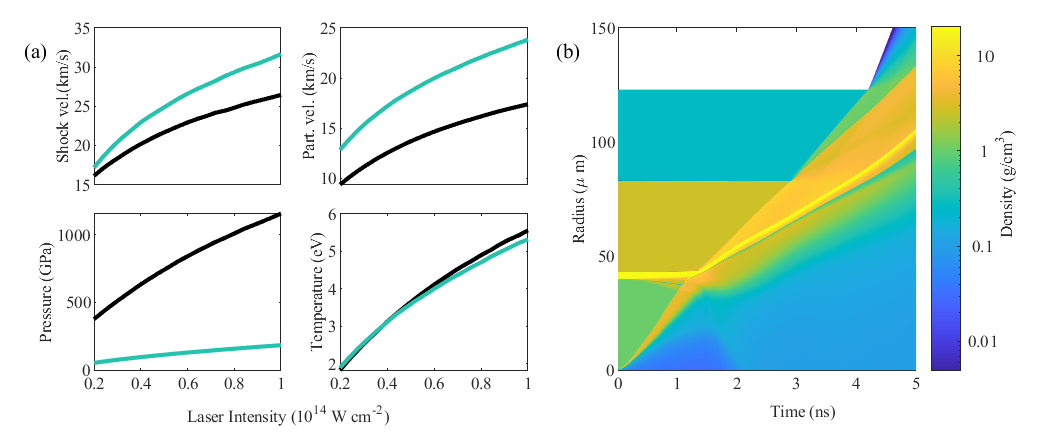
\includegraphics[width=1\textwidth]{figures/Experiment/PreExperimentHydro.eps}% Here is how to import EPS art
\caption{\label{fig:PreExpHydro} Shock conditions in the quartz (black) and foam (teal) as a function of intensity (a), and a density plot showing shock propagation through the target for an intensity of \num{1e14} \unit{\W\per\centi\meter\squared}. The quartz shock velocity informed decisions on the required etalons. The shock pressure in the quartz is also confirmed to be above the threshold for a reflective shock for the full range of simulated intensities.}
\end{figure}

Two-dimensional simulations of this setup were also performed to ensure that the shock was planar and that similar shock behaviour was observed in higher dimensions. The simulations presented in this section were performed in h2D (the two-dimensional version of Hyades). This is a Lagrangian code and as such suffers from mesh tangling, where the movement of the different zones can cause the mesh to become distorted and prevent the simulation from continuing. This requires the user to manually rezone the problem, and frequently also resulted in the simulation code crashing. After a number of iterations a sufficiently detailed simulation was ran to completion. Other 2D simulations were performed in Multi-2D and FLASH 2D by the other collaborators and were used to confirm these results; as these codes were ran with more success they were used instead of h2D for the post-shot simulations, and will be discussed in more detail in that section.

In h2D, a simple four layer target was simulated without a step in the foam. This was sufficient to measure shock propagation and to estimate the shock variables, as well as to indicate the shock planarity. 2D FLASH simulations (performed by other collaborators) were used to confirm that the step did not have a significant impact on the shock behaviour (this can be seen in later sections). h2D is an axisymmetric code, and so the target is simulated as a cylinder where the shock propagates along the long axis. R=0 is the axis of symmetry, and the 2D plane can be rotated around this axis to produce the full target (this also means that any applied beams are actually rings of laser light). 

The laser was simulated as 3 beams at -25$^{\circ}$, 0$^{\circ}$, and 25$^{\circ}$ to the target normal. Given the real experimental configuration (three pairs of two beams) a simulated setup consisting of two beams at 6$^{\circ}$ and -6$^{\circ}$ would also have been valid, but the three beam setup was chosen as it would give less 1D behaviour and thus represent a worst-case scenario. The laser beams are simulated by specifying a number of `rays' with an initial angle and position. The rays were created using a `random-to-uniform' lens-to-target mapping in Matlab. 10,000 uniformly spaced points were generated over the laser spot at the target, and for each point an incident ray was generated. Each ray was given an origin position at random, corresponding to a position on the lens for one of the three laser beams (considering the real lens size and lens-to-target distances). This method ensures that uniform illumination of the laser spot is achieved with the finite number of beams, while also using a random mapping to ensure behaviours such as defocussing past the laser focus. The energy of the ray was scaled according to the square it's radial position at the target; this accounted for the axisymmetric symmetry, and the fact that a ray incident on a higher radial position is spread over a much larger area if the 2D slice is converted to a 3D cylinder. A schematic showing the simulation setup is shown in Figure \ref{fig:H2DSchematic}

\begin{figure}[hbt!]
\centering
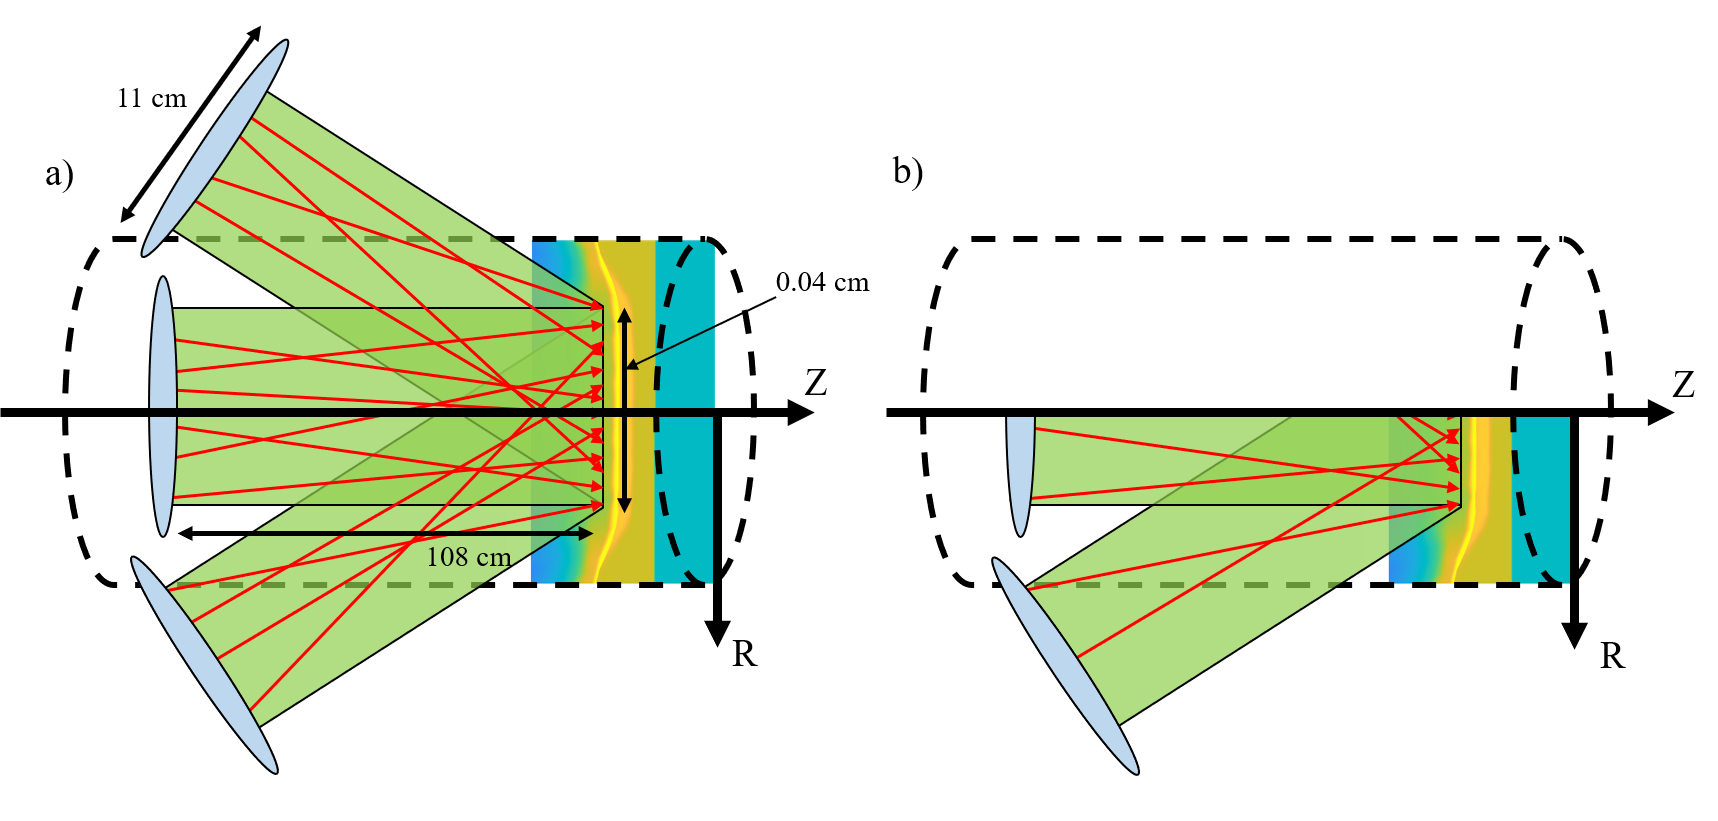
\includegraphics[width=1\textwidth]{figures/Experiment/H2DSchematic2.png}% Here is how to import EPS art
\caption{\label{fig:H2DSchematic} A schematic (not to scale) showing the simulated setup. In a), the full concept is shown. Three three beams produce a 400 \unit{\micro\meter} laser spot on the target. These beams are described by a series of rays originating from three 11 cm diameter lenses 108 cm from the target (these dimensions are accurate to the experiment). A small number of example rays are demonstrated by the red arrows. The rays are evenly spaced at the laser spot, but each is mapped to a random origin point on one of three lenses, which ensures the beam would defocus appropriately beyond the focal plane (the lenses are much larger than the focal spot, and so in practice these beams are heavily focussed - unlike in the schematic). For the purposes of the simulation, the target is considered to be a cylinder. R and Z are simulated, but the azimuthal behaviour is neglected (due to the 2D nature of the simulation). In b), the section included in the simulation is shown. Half the target diameter is simulated, and this can be extruded round the azimuth to produce the full target. Only the rays incident on this half of the target are included - but as the rays are specified at the target surface, it is possible to include rays that would have originated on the other side of the Z-axis. As the rays would also be uniform around the azimuth, the two off-axis beams would actually be simulated as a cone of incoming laser light.}
\end{figure}

Figure \ref{fig:H2DPlot} (a) shows four snapshots of the 2D shock structure. It can be seen that the shock front is relatively planar over a nearly 200 \unit{\micro\meter} radius (and thus the 400 \unit{\micro\meter} diameter of the imaged region). Figure \ref{fig:H2DPlot} (b) shows the shock propagation through the target (at the position of the dashed black lines in (a)) as a function of time, which shows good qualitative agreement with the 1D simulation seen in Figure \ref{fig:PreExpHydro}.

\begin{figure}[hbt!]
\centering
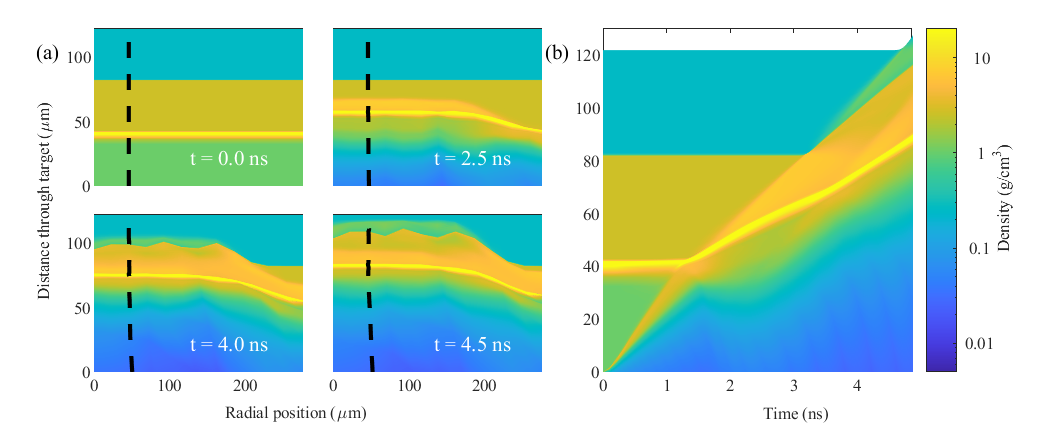
\includegraphics[width=1\textwidth]{figures/Experiment/H2DPlot.eps}% Here is how to import EPS art
\caption{\label{fig:H2DPlot} A two-dimensional h2D simulation of the setup using a simple four-layer target (ablator, gold, quartz and foam without the step structure), for a laser intensity of \num{1e14} \unit{\W\per\centi\meter\squared}. (a) shows four snapshots of the 2D simulation at the indicated times, while (b) shows the shock propagation of through the target as a function of time for a given radial position, represented by the black dashed lines in (a). It can be seen that for the later two times, the black dashed line is noticeably curved. This is because the lagrangian mesh moves as the simulation occurs, and thus the mesh points (where the simulation parameters are returned) do not have fixed radii. This small amount of curvature does not significantly affect the results - particularly as it is only seen in the ablated material significant behind the shock.}
\end{figure}

Figure \ref{fig:H2DPressure} shows how the pressure just behind the shock front in this simulation varies across the radius of the target. It is clear from the figure that, while the pressure reduces towards the edge of the target, over the central region the shock pressure is relatively planar in both the quartz and the foam. Meanwhile, Figure \label{fig:H2DTiming} displays the shock breakout times from the gold, quartz and foam layers. This again indicates that the shock is planar over the central region of the laser spot.

\begin{figure}[hbt!]
\centering
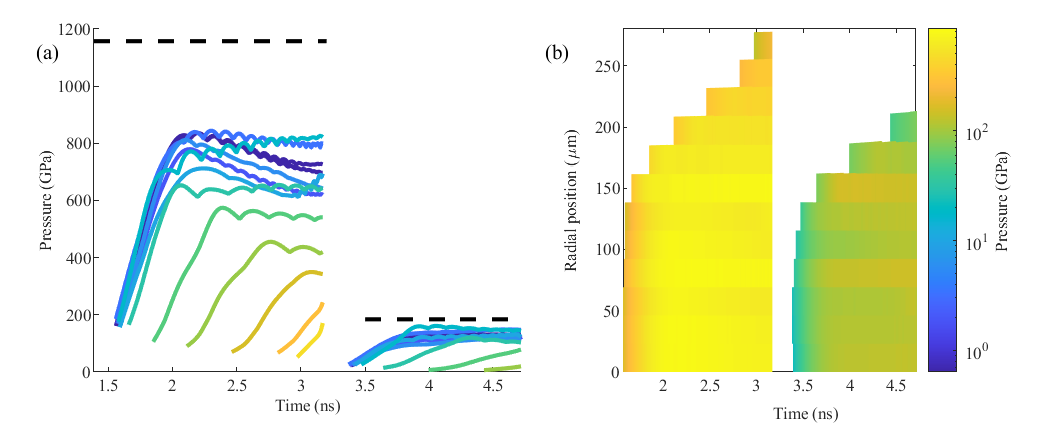
\includegraphics[width=1\textwidth]{figures/Experiment/H2DPressure.eps}% Here is how to import EPS art
\caption{\label{fig:H2DPressure} Plots showing the shock pressure in the simulation displayed in Figure \ref{fig:H2DPlot} as a function of both time and radial position. In (a), the different lines represent the different radial positions, with the colour transitioning from dark blue through to yellow (i.e. up the colour bar in Figure \ref{fig:H2DPlot}) as the radius moves further away from the center of the target. It can be seen here that the pressure is relatively uniform over the central regions, but drops off towards the edge. The dashed line represents the average shock pressure obtained in both materials in the 1D simulation. It is clear that this is significantly higher, but the difference appears to depend on simulation parameters (such as resolution) and was not observed in the other 2D codes. (b) represents the same data, but here the pressure is represnted by the colour on the 2D plot of position vs time. On both plots, the shock front pressure is only recorded when the shock front can be automatically identified in the simulation, and thus there are blank regions when the shock crosses material interfaces where the shock front is not clear.}
\end{figure}

\begin{figure}[hbt!]
\centering
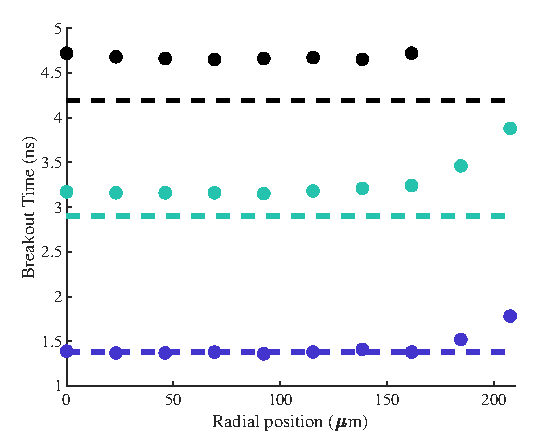
\includegraphics[width=0.6\textwidth]{figures/Experiment/H2DTiming.eps}% Here is how to import EPS art
\caption{\label{fig:H2DTiming} Shock breakout times from the gold (blue points), quartz (teal points) and foam (black points) as a function of radial position in the target. It can be seen that the breakout time is roughly steady over a radius of 150 \unit{\micro\meter}, and then increases towards the edge of the laser pulse. The dashed lines represent the breakout times obtained from the 1D Hyades simulation. While there is good agreement for the gold breakout, the 2D simulation returns a later breakout from the quartz and the foam, suggesting a slower and weaker shock. This is not observed in the other 2D simulations.  }
\end{figure}

Both Figure \ref{fig:H2DPressure} (a) and Figure \label{fig:H2DTiming} also compare these results to the 1D Hyades simulation shown in Figure \ref{fig:PreExpHydro}. It can be seen that the timing agreement is reasonably close, but there is a small increase in the shock transit time in both the quartz and the foam. This increase in transit time is due to a decreased shock velocity, which in turn indicates a lower shock pressure as seen in Figure \ref{fig:H2DPressure}. While the change in shock transit is relatively small, the corresponding impact on the pressure is relatively significant. Interestingly, as can be seen in the post-experiment simulations, such an effect was not observed to the same extent in the simulations performed in other 2D codes. This effect (particularly the pressure) was found to vary with the resolution of the simulations, suggesting it had not fully converged; unfortunately it was not possible (due to persistent issues with mesh tangling and crashing) to increase the resolution of the simulation to a point where the results converged. As such, while the h2D simulation was useful for confirming the shock planarity and expected behaviour in 2D, it was decided that the results should not be relied on for the precise shock timings/pressures, and the other codes (such as Multi and FLASH) were used for the post-experiment 2D simulations.


%were also performed in a variety of codes, to check that the shock was relatively consistent across the shock diameter. Simulations were performed in h2D (the 2D version of Hyades) which showed that the shock behaviour was largely similar to that seen in Hyades. The shock was planar over most of the 400\unit{\micro\meter} imaged region, and the transit time was only slightly reduced compared to the 1D simulations. Piotr R\k{a}czka also performed a 2D Flash simulation which included the target step (as h2D was a lagrangian code, issues with mesh tangling prevented such a simulation from being performed) and showed that this did not significantly affect the shock propagation.

\section{Changes and adaptations during the experimental run}

Challenges that arose during the six-week experimental run necessitated a variety of changes to the initial experimental plan. In this section, these changes (and the issues that inspired them) are discussed.

\subsection{Changes from planned target} \label{Target issues}
The actual targets that were delivered for the experiment differed slightly from the planned targets. This was due to challenges in fabricating the targets, as well as one of the suppliers failing to deliver a shipment of quartz (which also limited the number of available targets).
\begin{itemize}
    \item \textbf{Different target dimensions}: the delivered quartz was thicker than expected, which led to the quartz layer in each target being $\sim$ 50 \unit{\micro\meter} thick (rather than the planned 40 \unit{\micro\meter}). The foam thickness also varied, and was frequently significantly larger than the planned 40 \unit{\micro\meter}.
    \item \textbf{Fewer targets with an AR coating}: the reduced quantity of quartz meant that some targets did not have the planned anti-reflection coating. Fortunately, this did not seem to have a significant effect.
    \item \textbf{Delamination in some targets}: in a small number of early targets, the ablator/gold delaminated from the quartz, and had to be glued back on. The glue layer prevented an accurate timing measurement in the quartz and meant that the target could not be used for impedance matching; however, they were shot as test/setup targets. These later became important in understanding some features of the results (see Section \ref{Glue targets}).
\end{itemize}

\subsection{Poor VISAR illumination and subsequent changes to optical setup}

Once setup was complete and shots started, it became apparent that the probe laser was only illuminating a small section of the imaged region. This prevented sufficient VISAR data from being collected. This was due to the fact that the probe laser travelled through the optical relay before reaching the target, which demagnified it and brought the laser to focus at the target position, as seen in Figure \ref{fig:Full experiment schematic}. 

An initial solution was to place a 700 \unit{\milli\meter} focal length lens between the laser and the VISAR beamsplitter; this would mean the laser was not collimated when entering the relay, and so would not be perfectly focussed by the objective lens. This did not sufficiently improve the problem. As such, a modified setup was designed which would solve the problem while requiring minimal changes to the optical relay (which at this point was already setup). In the new setup, the first mirror after the objective lens was replaced with a beamsplitter, and the probe laser was injected through this beamsplitter rather than after the VISARs. This meant the probe laser bypassed the relay, and only the objective lens was shared. A lens was placed in the probe laser beampath prior to this beamsplitter to form a lens pair with the objective lens; this meant that the probe laser would be collimated by the objective lens, and thus collimated when it reached the target \footnote{While this was initially the case, extra mirrors were later added to the setup to give additional control one the probe laser position. Spatial constraints meant these mirrors had to be added between the lenses, which increased the P1-L1 distance from the intended 550mm to 875mm. This meant that the beam was no longer perfectly collimated. However, burn paper tests showed that the spot size at the target position was still sufficient, and the illumination remained uniform. Simulation of this setup with the ray tracing code suggested the spot size was around 1 mm in diameter.}. A schematic showing this new setup can be seen in Figure \ref{fig:Full experiment schematic with new laser setup}, and a full CAD model of this updated setup (produced by the CLF CAD team) is shown in \hl{FIGURE}.

\begin{figure}
\begin{centering}
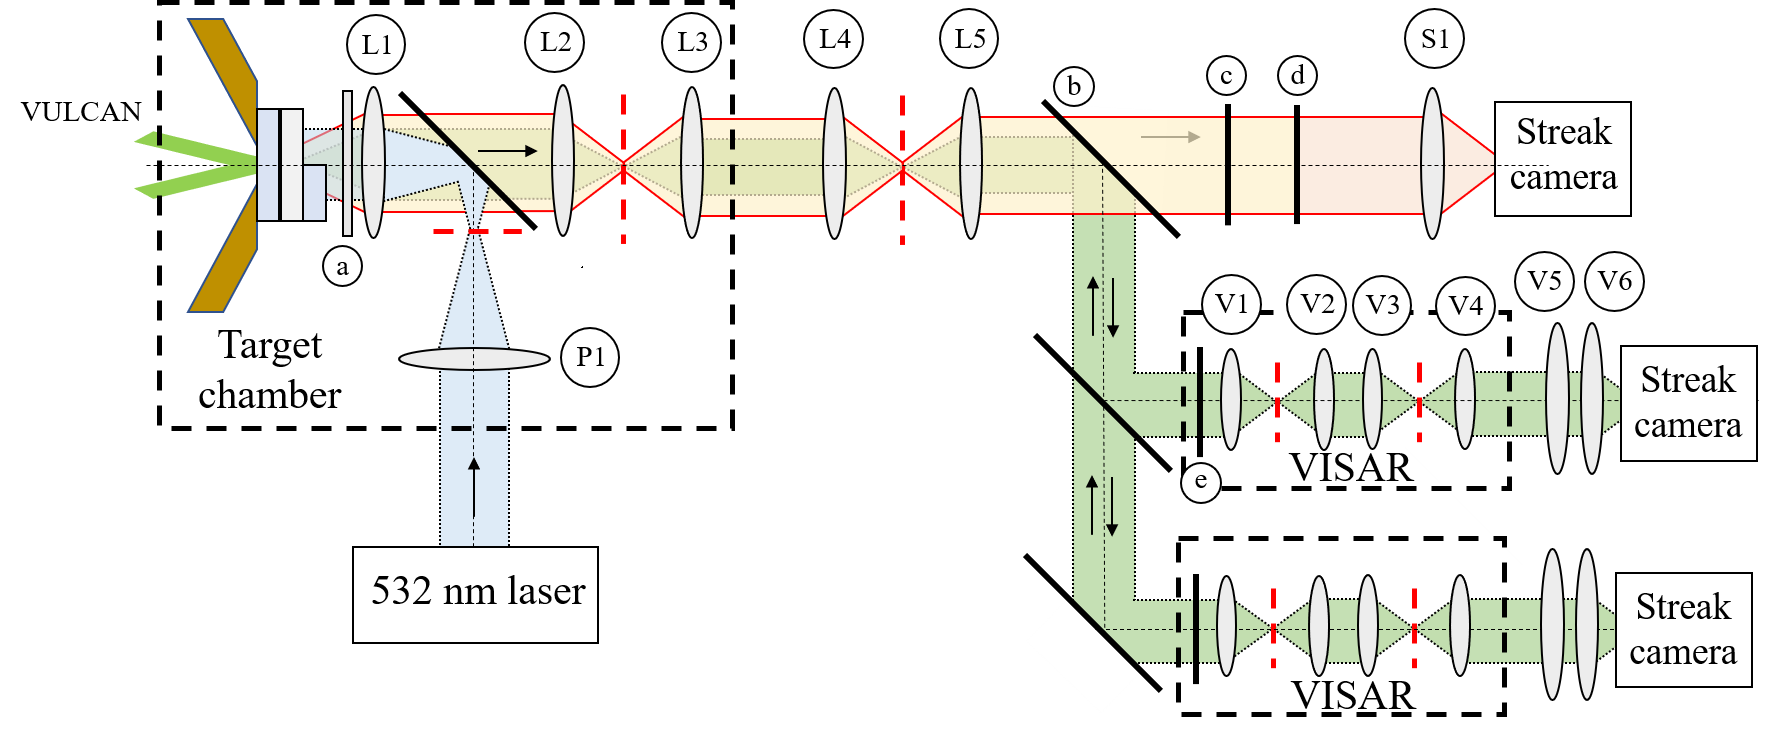
\includegraphics[width=1.0\textwidth]{figures/Experiment/Full experiment schematic new laser injection.png}% Here is how to import EPS art
\caption{\label{fig:Full experiment schematic with new laser setup} The full schematic, with the new probe laser injection. The probe laser is displayed in blue to differentiate the beampath from the reflected probe light shown in green, but both have the same 532 nm frequency. The labels are unchanged from Figure \ref{fig:Full experiment schematic}, except for a new 400 mm lens P1. This forms a lens pair with the objective lens L1; the beam passes through P1 and is focussed at the focal point of L1, so that L1 collimates the beam before it reaches the target. The incoming laser is then scattered from the target, and the objective lens is thus still considered to be collimating the reflected light. The only other changes from the original setup are the addition of a beamsplitter between L1 and L2 (replacing a mirror in the previous setup), and the replacement of the beamsplitter prior to the bottom VISAR with a mirror.}
\end{centering}
\end{figure}

This setup significantly improved the illumination, as shown in Figure \ref{fig:VISAR before and after}. The downside of this approach was that the beamsplitter in the relay would reduce the intensity of the captured emission (both the VISAR signal and the self-emission) by half (although the second VISAR beamsplitter could be replaced with a mirror, which compensated for the signal loss on one of the VISARs). This was a necessary sacrifice though, as without this change the illumination was not sufficient for the VISAR to be used.

\begin{figure}
\begin{centering}
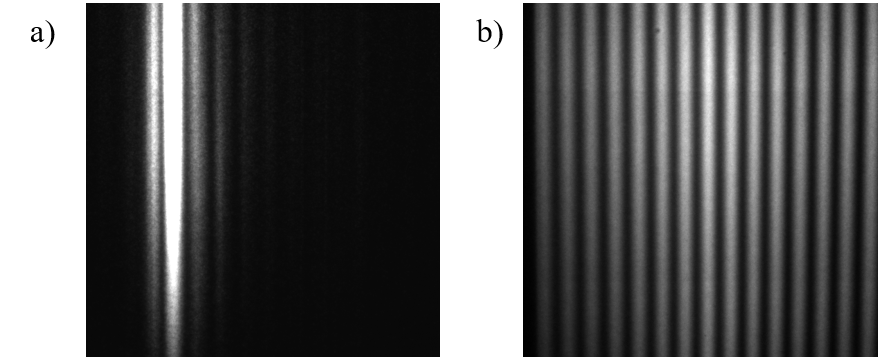
\includegraphics[width=0.8\textwidth]{figures/Experiment/VISAR before and after.png}% Here is how to import EPS art
\caption{\label{fig:VISAR before and after} Images taken in focus mode on the VISAR streak camera from a piece of quartz a) using the original setup and b) using the updated setup. The quartz sample is stationary, and the camera used in focus mode so the signal at a single time across two spatial dimensions is recorded; uniform fringes are expected across the whole image. It is clear that in (a) only part of the sample is well-illuminated, whereas the new setup well illuminates the full imaged region. The signal strength was also better using the new setup; (a) is only brighter due to different filtering.}
\end{centering}
\end{figure}

\subsection{Later than expected shock breakout times}

It was noted mid-experimental run that the shock breakout times being measured for a given intensity were significantly longer than those predicted by simulations. This meant that the VULCAN drive beam was frequently ending prior to shock breakout - contrary to the experimental plan, where the drive beam would be kept on until shock breakout to ensure a sustained shock. Additional simulations were therefore performed mid-run to determine the expected impact of the drive laser pulse ending before shock breakout time. It was found that in fact this did not lead to substantial differences in shock behaviour, and thus this was not a major cause for concern.

\subsection{Signal strength issues}

Throughout the experiment, both diagnostics suffered from a lack of signal strength. Some of this could be explained by the streak cameras. Three were used in this experiment; two high dynamic range Hamamatsu C7700 cameras were used for the VISARs, while a Hamamatsu C5680 was used for the streaked optical pyrometer. The older C5680 was expected to be less sensitive, and this was used for the SOP accordingly (as the VISAR was the more important diagnostic). This camera struggled for signal throughout. One of the VISARs also consistently recorded low signals compared to the other; it was later realised that this camera had an S1 streak tube as opposed to the S20 used in the other. The S1 tube (which was also present in the SOP streak) is around two orders of magnitude less sensitive to 532 \unit{\nano\meter} light.

The signal strength for both VISARs was also heavily influence by the probe laser. This laser was relatively high power, and significant ND filters were needed to prevent it damaging the optics in the optical chain. However, the long optical relay likely resulted in some decrease in signal strength. There were also significant operational issues with the probe laser. It frequently did not seed, resulting in the pulse being significantly weaker, and being emitted at a different time. This would occur on shots, where the low strength and change in time (relative to the VULCAN pulse) would prevent useful data from being collected. After attempting a number of fixes, the facility staff eventually replaced the seed laser within the unit with one from a different laser. This improved the situation and allowed the experiment to continue, but the timing and pulse intensity continued to vary drastically from shot to shot.

\section{Data analysis: VISAR}
The analysis of the raw experimental data, leading to the published results, required a number of steps and methods to be applied - these are outlined in sequence in this section. In order to do this, I wrote a large amount of Matlab code to automate a number of processes, and (where user-selections had to be made) to save these choices. This meant that the data can be returned to later on to see the decisions that were made, and to aid repeatability.

\subsection{Collected data for a typical shot}

The data collected for a typical shot is consisted of:
\begin{itemize}
\item Photos of the target (taken by target fabrication)
\item Measurements of the target dimensions (performed by target fabrication)
\item Measurements of the energy of each beam (from the on-shot calorimetry)
\item Traces of the pulse profile of the beams (taken from photodiodes viewing parasitic signal from a lossy-mirror)
\item Images from each VISAR streak camera (one from each, two in total)
\item Image from the SOP streak camera (one - containing fiducial signal from start of beam)
\end{itemize}

\subsection{Identifying shock velocities from raw VISAR data}

In the VISAR streak images, the x-axis position is a spatial dimension, and the image contains two distinct halves - one corresponding to the quartz, and the other to the foam. The y-direction represents time, with later times at the bottom of the image. A labelled example can be seen in Figure \ref{fig:VISARImage}. Three `transitions' can be identified in the image. Firstly, shock entry into the quartz can be identified by a sudden change in signal intensity on the quartz half of the image. Secondly, shock breakout from the quartz rear-surface can be identified by fringe extinction on this half. This also corresponds to the shock entering the foam (although as the foam is opaque to the probe laser, no change is seen in the foam signal at this point). Finally, shock breakout in the foam could also be identified by shock breakout, but on the other half of the image.

\begin{figure} [h]
\begin{centering}
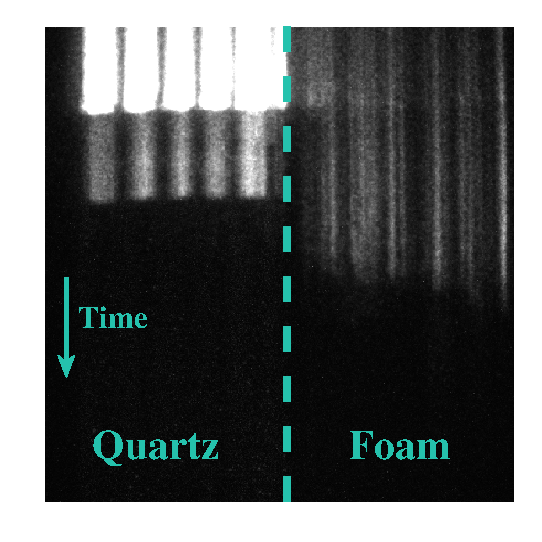
\includegraphics[width=0.5\textwidth]{figures/Experiment/VISARImage.eps}% Here is how to import EPS art
\caption{\label{fig:VISARImage} A raw VISAR streak image, labelled to indicate the quartz and foam signals. Three clear changes can be observed; a change in fringe intensity in the quartz (corresponding to the shock entering the quartz from the gold), fringe extinction in the quartz (shock breakout from the quartz), and fringe extinction in the foam (shock breakout from the foam). }
\end{centering}
\end{figure}

Both VISAR images were viewed side by side, and the contrast adjusted to aid identification of these changes. On each image, where possible, the three times were selected. The selections used for a particular shot are displayed in Figure \ref{fig:VISAR ROI}. As the change in signal was not always instantaneous, a `region of interest' (ROI) was selected to cover the full range over which the transition most likely occurred. These selections for each transition, image, and shot were saved and stored.

\begin{figure} [h]
\begin{centering}
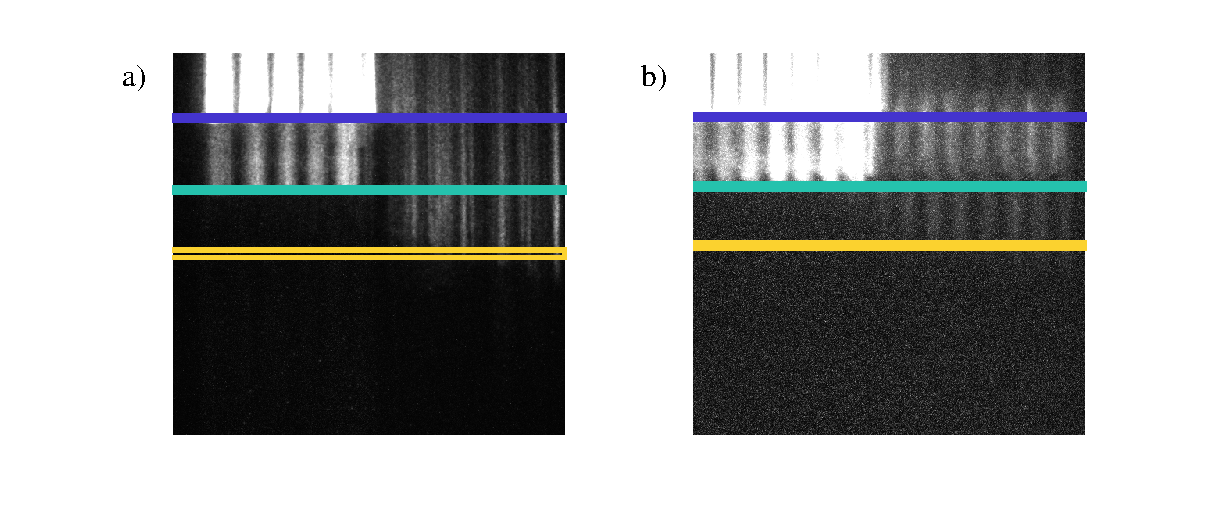
\includegraphics[width=1.0\textwidth]{figures/Experiment/VISARROI.eps}% Here is how to import EPS art
\caption{\label{fig:VISAR ROI} VISAR images from the two VISARs for the same shot. The selected regions where the shock transitions are believed to be confirmed are shown. The blue region corresponds to shock entry into the quartz, while the teal region corresponds to shock breakout from the quartz and the yellow corresponds to shock entry into the foam. The edge of image (a) appears to show some curvature; this is expected based on the simulations due to the size of the VULCAN laser spot. The region was chosen to capture the transition at the center, where the shock seems to be more planar.}
\end{centering}
\end{figure}

The streak time was taken from the shot sheet, and used to convert the pixels (in the y-direction) to time. The ROI's were thus converted from a pixel range into a time (the mean position of the window) with associated uncertainty (the width of the window). The finite slit width of the camera also introduced a minimum possible time resolution (which was used for the uncertainty if the ROI width was less than this value). The shock transit times through both quartz and foam were then calculated, as the differences between these three transitions.

The two VISARs, when both operating well, gave independent measurements of the same behaviour. In many cases, each transit time could only be confidently identified from one of the two VISARs - in such cases, only the transit times from a single image were used. However, in cases where both VISARs returned good data, the calculated transit times from the two diagnostics were combined were combined. Since the value from both should be consistent, having two measures allowed the error to be reduced. The 'average' measurement range was taken as the region in which the two seperate measurements overlapped.

Finally, the thickness of the quartz and foam layers (with estimated uncertainties) then used to calculate the average shock velocity in each material.

\begin{figure} [h]
\begin{centering}
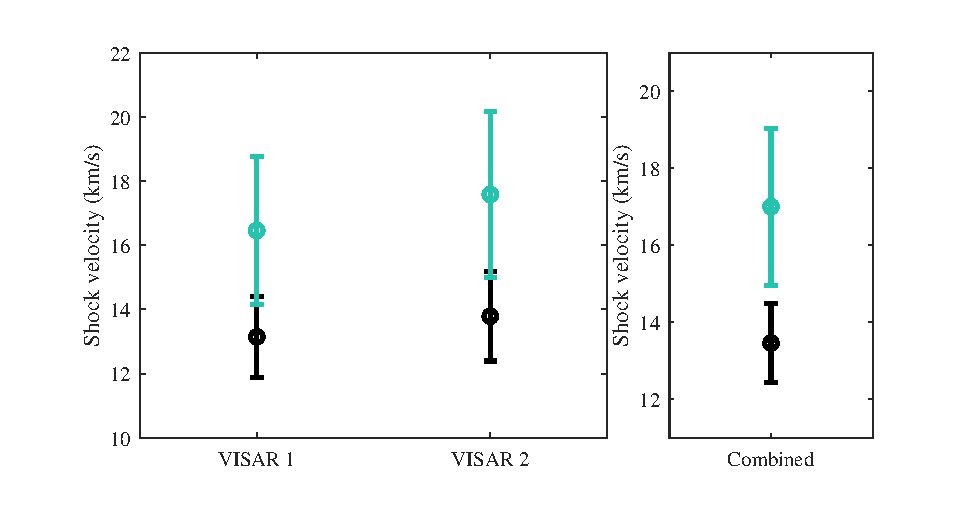
\includegraphics[width=1.0\textwidth]{figures/Experiment/VISARTiming.eps}% Here is how to import EPS art
\caption{\label{fig:VISAR Timing} Calculated shock velocities in the quartz (black) and the foam (teal) using the shock timings obtained from the VISAR images in Figure \ref{fig:VISAR ROI}. In this shot, all three timings can be identified from both VISARs. The shock velocities corresponding to the timing data from each of the two VISARs independently is displayed, along with the shock velocity calculated from the `combined' timings. The combined measurement uses both sets of VISAR measurements to reduce the error, giving a `combined' set of possible timings that is compatible with the range measured by each VISAR.}
\end{centering}
\end{figure}

An attempt was made at this point to identify the same three tranistions from the SOP data, to provide another measure of these shock transit times. However, this turned out not to be possible - there was no clear change in the SOP data correlating to the shock breakout from the quartz, which prevented either shock breakout time from being calculated. It was also found that the start of the foam self-emission occurred before the shock breakout in the VISAR images (likely indicating some transparency of the foam to these self-emitted frequencies).

\subsection{Confidence ranking of shots}
Although 68 shots were used in total, far fewer of these resulted in VISAR images where all three necessary transitions could be confidently identified. Often it was not possible to select a particular breakout time from the VISAR data, or it was unclear if there was really a change in signal there. To account for this, a confidence ranking of each shot was performed as the data was analysed.

Each shot was given a score between 0 and 10. A 10 meant that it was absolutely certain that the times identified corresponded to those signals. A 0 meant that there was no timings which could be determined. A 5 was used as the threshold - meaning that I believed that someone else performing the analysis would be expected to choose the same times as me. This included a range of factors. Agreement between the two VISARs resulted in higher confidence. Strange artefacts or behaviours in the signals led to lower confidence (as did unreasonable calculated values). This was an iterative process, which was returned to with later information (such as evidence of second shocks, or cross-comparison with SOP data). For the final results only data with a confidence value greater than 5 were used, which removed shots where there was low confidence that real behaviours were being measured.

\subsection{Impedance matching calculation} \label{IM calc}
The impedance matching calculation was then performed to calculate the foam shock state from the two shock velocity measurements. The principle of this calculation is described in \hl{SECTION}.

A common approximation in impedance matching calculations is not to calculate the release isentrope accurately, but instead to reflect the hugoniot of the reference material (for this experiment, quartz) around the reference material (quartz) shock state. For low pressures this is reasonably accurate, but it can introduce errors as the pressure is increased. An initial calculation was performed using this approach to produce a first estimate of the results, and to provide a sanity check on the results of the more complicated (but more complete) approach. In this calculation, the Hugoniot described in \cite{Knudson2009} was used: \begin{equation} \label{eqn:Hugoniot} U_s = \sum_{n=0}^3 a_n u_p^n \;, \end{equation} with coefficients in Table \ref{tab:HugoniotCoeffs} \cite{Knudson2013} - a cubic fit to experimental data from \cite{Knudson2009} The intercept of this Hugoniot with the quartz Rayleigh line,  $P = \rho_0^{quartz} U_s^{quartz} u_p$, where $P$ is Pressure, $u_p$ is particle velocity, and $U_s^{quartz}$ is the measured quartz shock velocity, was found. This intercept provided ($P^{quartz}, u_p^{quartz}$), the quartz shock state. The Hugoniot was then reflected around this point to approximate the release isentrope. The intercept of this reflected Hugoniot with the foam Rayleigh line, $P = \rho_0^{foam} U_s^{foam} u_p$, was then found, which defined the foam shock state ($P^{foam}, u_p^{foam}$). This was performed for each shot.

\begin{table}%The best place to locate the table environment is directly after its first reference in text
\centering
\caption{\label{tab:HugoniotCoeffs}%
Coefficients for the quartz Hugoniot in equation \ref{eqn:Hugoniot}, reproduced from \cite{Knudson2013}.
}
\begin{tabular}{lccr}
\hline\hline
\textrm{$a_0$ \si[per-mode=symbol]{(km/s)}}&
\textrm{$a_1$}&
\textrm{$a_2$ \si[per-mode=symbol]{\kilo\meter\per\second} }&
\textrm{$a_3$ \si[per-mode=symbol]{(km/s)^{-2}} } \\
\hline
1.754 & \num{1.862} & \num{-3.364E-2} & \num{5.666E-4}\\
\hline\hline
\end{tabular}
\end{table}

The calculation was then performed using a complete calculation of the release isentrope. This calculation used a slightly different functional form for the Hugoniot, which was better suited to the impedance matching calculation. The release isentrope was calculated largely according to the method of \cite{Knudson2013}, but with a few small differences. In their paper, Knudson and Desjarlais model the isentrope using a new `linear-reference' Mie-Gruneison model. The key part of this model is that the Gr{\"u}neisen parameter is variable, which results in reduced errors. However, the range of pressures over which this model is valid does not extend across those achieved in this experiment, and the model returns non-sensical results for some of these values. Their paper compares to the previous standard - a conventional Mie-Gruneison model, with a fixed Gr{\"u}neisen parameter of $\Gamma = 0.64$, and this was instead used in this analysis. The calculation follows that described for the reflected-Hugoniot model, except that once the quartz shock state ($P^{quartz}, u_p^{quartz}$) has been found, the associated isentrope for that state is calculated following the method described in appendix. This is then used in place of the reflected Hugoniot. Once this had been performed for all shots, the results of this calculation were compared to the reflected hugoniot ones, and the difference was found to be negligible.

\begin{figure} [h]
\begin{centering}
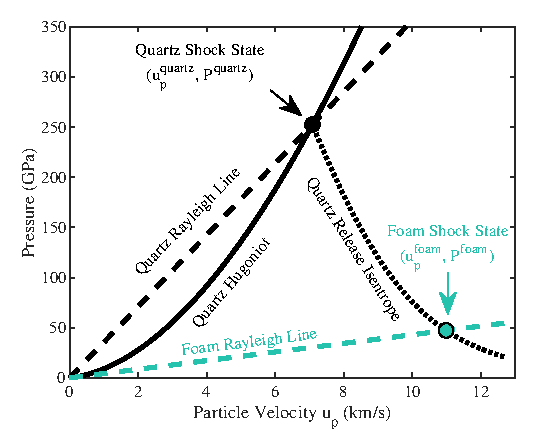
\includegraphics[width=0.6\textwidth]{figures/Experiment/ImpedanceMatch.eps}% Here is how to import EPS art
\caption{\label{fig:Impedance Match} The impedance matching calculation for the shock velocities obtained in Figure \ref{fig:VISAR Timing}. The intercept of the quartz Rayleigh line and the quartz Hugoniot defines the quartz shock state. The release isentrope for this shock state is then calculated, and the intercept of this curve with the foam Rayleigh line describes the foam shock state.}
\end{centering}
\end{figure}

\subsection{Uncertainty quantification - Monte Carlo analysis} \label{MC error}

Uncertainty quantification for the shock variables obtained using the impedance matching calculation was performed using a Monte Carlo approach. This technique allowed the experimental uncertainty to be propagated through the complex IM calculation, while also allowing including uncertainty contributions from the quartz hugoniot fit and foam initial density. This section is accompanied by a flow chart in Figure \ref{fig:MC Flow Chart} which shows the different steps of the calculation for the shot considered in the previous sections, with the relevant distributions and example MC samples. Uncertainty quantification in this way has previously been performed on other similar experiments.

%My initial solution to this problem was to perform each calculation three times for a single shot. Consider the IM calculation as a black box, which takes inputs (shock velocities) and returns outputs (shock pressures, particle velocities etc.). If we take an input of $A \pm B$, the calculation was performed for A, A + B, and A - B. This would return answers of C, D, and E - where C is the 'value' we would then use, and D and E are the ranges of our uncertainties. This approach worked, but lacked elegance. It was difficult to include Hugoniot error, and it also required careful thought to ensure the right 'sets' of inputs were included to make sure the uncertainties summed in the right way. This approach also had statistical flaws - I was finding max errors by assuming that each input had it's maximal error at the same time (a worst-case scenario), but this is more pessimistic than standard error propogation formulas, and thus led to larger errors.

The calculation begins with the measured shock velocities for the quartz and foam for a particular shot. These are of form $U_{shock} \pm \epsilon$; a quoted value $U_{shock}$, with an experimentally measured error that is symmetric around this value $\epsilon$. A normal distribution is then produced for each of the two shock velocities; this has a mean at the value $U_{shock}$, and a standard deviation of $\epsilon$. A similar distribution is produced for the foam initial density.

These distributions were then used to perform 10,000 Monte Carlo iterations of the impedance matching calculation for each shot. For each iteration, a sample is randomly generated for each shock velocity and the foam density according to the relevant distribution. Samples are also generated for each of the four Hugoniot fit parameters, according to the covariance matrix covariance matrix\footnote{The printed matrix is that provided by \cite{Knudson2013}, but actually attempting to use this to generate the parameters returned an error due to the matrix not being positive definite. To resolve this, a small correction was added, $C + \num{1e-10}\cdot I$ was required, where $I$ is the identity matrix \cite{Holton2003}.}  provided in \cite{Knudson2013},

\[C = 
\begin{bmatrix}
\num{2.097e-2} & \num{-6.159e-3} & \num{5.566e-4} & \num{-1.572 e-5}\\
\num{-6.159e-3} & \num{1.877e-3} & \num{-1.742e-4} & \num{5.017e-6}\\
\num{5.566e-4} & \num{-1.742e-4} & \num{1.650e-5} & \num{-4.834e-7}\\
\num{-1.572 e-5} & \num{5.017e-6} & \num{-4.834e-7} & \num{1.438e-8}\\
\end{bmatrix}. 	
\]

The impedance matching calculation was then performed, as described in Section \ref{IM calc}, using these randomly sampled values. The 10,000 iterations therefore produced 10,000 different estimates of the quartz and foam shock states, providing distributions of each of the relevant shock variables. The standard deviations $\sigma$ of these distributions were then calculated, and used to define the uncertainty range of these values.


%\begin{table}%The best place to locate the table environment is directly after its first reference in text
%\caption{\label{tab:HugoniotCovariance}%
%Coefficients for the quartz Hugoniot in equation \ref{eqn:Hugoniot}, reproduced from \cite{Knudson2013}.
%}

%\begin{tabular}{lccccccccr}
%\hline\hline
%\begin{tabular}{@{}c@{}}$\sigma_{a_0}^2$ \\ $(\times 10^{-2})$\end{tabular}
%\begin{tabular}{@{}c@{}}$\sigma_{a_0}\sigma_{a_1}$ \\ $(\times 10^{-3})$\end{tabular}
%\begin{tabular}{@{}c@{}}$\sigma_{a_0}\sigma_{a_2}$ \\ $(\times 10^{-4})$\end{tabular}
%\begin{tabular}{@{}c@{}}$\sigma_{a_0}\sigma_{a_3}$ \\ $(\times 10^{-5})$\end{tabular}
%\begin{tabular}{@{}c@{}}$\sigma_{a_1}^2$ \\ $(\times 10^{-3})$\end{tabular}
%\begin{tabular}{@{}c@{}}$\sigma_{a_1}\sigma_{a_2}$ \\ $(\times 10^{-4})$\end{tabular}
%\begin{tabular}{@{}c@{}}$\sigma_{a_1}\sigma_{a_3}$ \\ $(\times 10^{-6})$\end{tabular}
%\begin{tabular}{@{}c@{}}$\sigma_{a_2}^2$ \\ $(\times 10^{-5})$\end{tabular}
%\begin{tabular}{@{}c@{}}$\sigma_{a_2}\sigma_{a_3}$ \\ $(\times 10^{-7})$\end{tabular}
%\begin{tabular}{@{}c@{}}$\sigma_{a_3}^2$ \\ $(\times 10^{-8})$\end{tabular} \\
%\hline
%2.097 & -6.159 & 5.566 & -1.572 & 1.877 & -1.742 & 5.017 & 1.650 & -4.834 & 1.438\\
%\hline\hline
%\end{tabular}
%\end{table}


10,000 Monte Carlo iterations were then performed. For each iteration, a random sample was taken from each distribution. The impedance matching calculation was then performed using this random set of values. Overall, this produced 10,000 different calculated quartz and foam shock states, giving distributions of each output value (i.e. quartz/foam pressures, particle velocities etc.). The uncertainty of each of these parameters was taken as the standard deviation of the corresponding distribution.

An interesting detail of this calculation is that the distribution mean does not always equal the value obtained if the IM calculation is performed without considering uncertainty (i.e. if no MC sampling is performed, and thus for all shock velocities $U_{shock} \pm \epsilon$ the values of $U_{shock}$ are used, along with the exact Hugoniot fit parameters quoted in Table \ref{tab:HugoniotCoeffs} - this will henceforth be referred to as the `exact' IM calculation). This was most noticeable for the shock pressure, where there is a noticeable small amount of skew in the distribution (the particle velocity distributions are effectively normal). This effect arises from a non-linearity in the calculation. Consider a shock velocity $U_{shock}$ and associated pressure $P$. If there is a small positive increase in $U_{shock}$, this results in a larger change in $P$ than if there is a small decrease in $U_{shock}$ - leading to a distribution mean that is skewed towards higher values.

The most natural way to present the results of this calculation would be to quote each shock variable as the MC mean plus/minus the standard deviation. This could lead to confusion however - for instance, the quartz shock state would then be quoted as $\bar{u_p}^{quartz} \pm \sigma_{u_p^{quartz}}$ and $\bar{P}^{quartz} \pm \sigma_P_{quartz}$ (where a variable with a bar is used to indicate the MC distribution mean), but the state ($\bar{u_p}^{quartz}, \bar{P}^{quartz}$) would not actually be a valid state on the quartz Hugoniot. To avoid this, the shock variables are instead quoted as the `exact' values - those obtained if the IM calculation is done without random sampling of any of the variables. These values are quoted with asymmetric error to describe the same uncertainty range as the standard deviation (which was symmetric about the mean). This is shown in the last box of Figure \ref{fig:MC Flow Chart}, where one standard deviation $\sigma$ from the mean (solid black line) is described by asymmetric errors $\epsilon_+$ and $\epsilon_-$ around the `exact' quoted value (orange) (It is also worth noting that the difference between the mean and the exact value is relatively small, and this uncertainty range actually represents 34\% (i.e. $1 \sigma$) of the generated MC samples in either direction from the `exact' value to within one or two percent).

%While the resulting distributions for the particle velocity were effectively normal, there was some noticeable skew in the Pressure distribution. This meant that the mean of the distribution was different to the value obtained for an `exact' impedance match calculation (note: in this case, `exact' is used to mean that for a shock velocity $U_{shock}$ with uncertainty $\epsilon$, quoted as $U_{shock} \pm \epsilon$, the calculation is performed for a value of $U_{shock}$ using the hugoniot parameters quoted in \label{tab:HugoniotCoeffs}). This difference is due to the non-linearity of the calculation; and indeed, an individual sample that used the `exact' shock velocities and Hugoniot parameters would return the exact outputs. Consider the exact pair $U_{shock}$ and $P$. If there is a small deviation $+ \delta$ from $U_{shock}$ in the positive direction, the resulting deviation from $P$ is larger than if there is a small deviation $- \delta$ in the negative direction. This shifts the mean to higher values. It is also worth noting that, as the number of MC samples tends towards infinity, the median of the MC samples tends towards the exact values. 

%Using the mean of the distributions would result in quoted values that were not consistent with the `exact' Hugoniot (i.e. the quoted ($P^{quartz}, U_s^{quartz}$) would not actually lie on the Hugoniot given by the quoted parameters in Table \ref{tab:HugoniotCoeffs}). To avoid this inconsistency, the `exact' value of each variable was used when quoting values - and so the values reported in the results section are those that would be achieved if the exact impedance matching calculation is performed on the quoted shock velocities. However, the calculated uncertainty - being the standard deviation of the distribution - is centered on the distribution mean, rather than this exact value. This means that the error bars that accompany the quoted values are asymmetric, as they are centered on the mean, rather than the `exact' value. These error bars still represent 34\% (i.e. $1 \sigma$) of the generated MC samples in either direction from the `exact' value to within one or two percent.

\begin{landscape}
\begin{figure} 
\begin{centering}
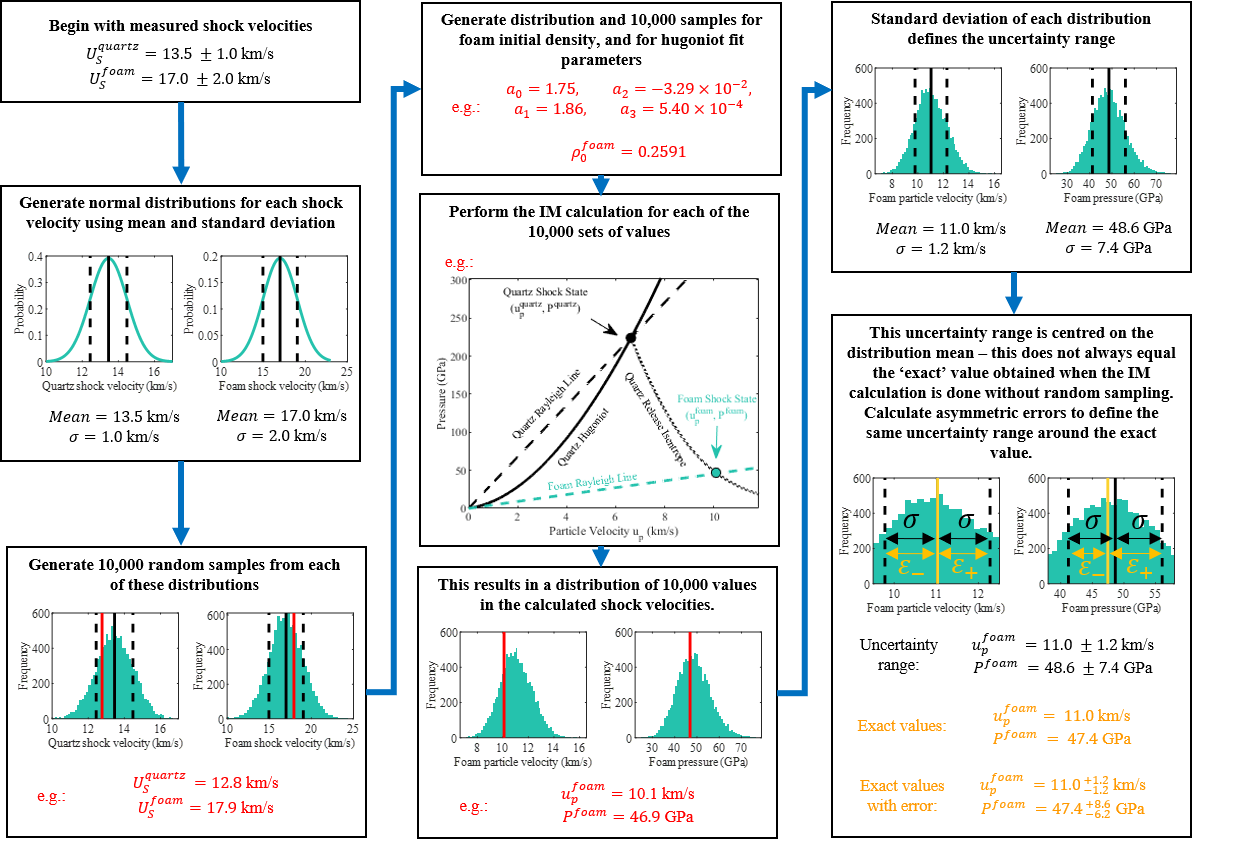
\includegraphics[width=1.5\textwidth]{figures/Experiment/FlowChart.png}% Here is how to import EPS art
\caption{\label{fig:MC Flow Chart} Flow chart showing the MC methodology for quantifying the uncertainty in the calculated variables. The MC analysis is shown for the same shot as the previous figures. The values/lines if red show the analysis performed for a single example set of the 10,000 random samples.}
\end{centering}
\end{figure}
\end{landscape}

\subsection{Calculation of velocity from VISAR fringe curvature}

The intention for this experiment was that the VISAR signal would display fringe motion in the quartz, and the quartz shock velocity as a function of time could be calculated from this following the analysis procedure described in \hl{SECTION}. Unfortunately this was mostly not possible; very few shots displayed any fringe motion, and even those that did had low signal strength or were too noisy for meaningful analysis to be conducted.

Attempts were made to perform this analysis where some curvature was observed. The analysis script produced by Dan Eakins expected full fringe motion; I adapted this so that it could instead be used to analyse just a small section of the VISAR data where motion was observed. As we did not have two VISAR signals of sufficient quality for each shot for unambiguous velocity determination, the correct velocity signal was estimated from the knowledge of the average velocity.


The clearest shot is presented in \hl{figure}. This indicates that the shock is reasonably stable, although some shock decay was observed. Unfortunately, limited conclusions could be drawn from this data.

\subsection{Calculating grey-body temperature from SOP data}
As for the VISAR streak images, the x-dimension in the SOP streak image was spatial, while the y-dimension was temporal. The streak time for the camera on each shot was used to convert pixels in the direction into time values. An example SOP streak camera image (for the same shot considered in the previous sections) is displayed in Figure \ref{fig:SOP data}

\begin{figure} [h]
\begin{centering}
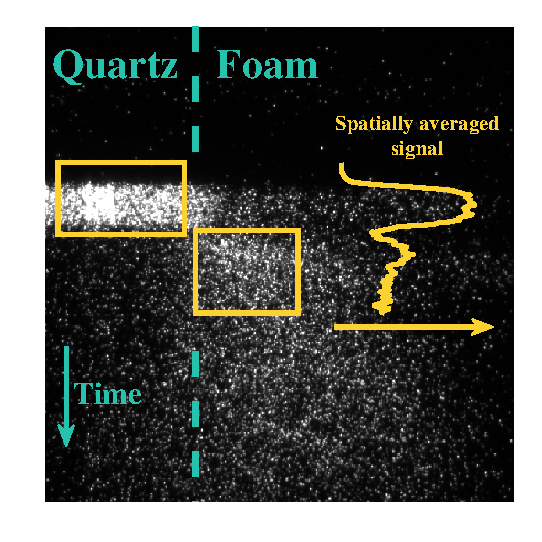
\includegraphics[width=0.6\textwidth]{figures/Experiment/SOPImage.eps}% Here is how to import EPS art
\caption{\label{fig:SOP data} SOP streak image. As with the VISAR image, the quartz is positioned on the left of the image, with the foam on the right. Time increased in the negative y-direction. The yellow rectangles represent the chosen regions covering the SOP emission for both materials, while the traces show the spatially averaged signal across these regions.}
\end{centering}
\end{figure}

In each image, a region was selected covering the emission from each material. This region was used for spatial averaging of the signal, to obtain an average intensity vs time for each material; this was chosen to cover the section of the image where the emission was uniform (i.e. to avoid including weaker signal in the averaging from the edge of the target), while being as wide as possible to improve the averaging. The maximum in the averaged signal for the two materials were then identified, and used in the temperature calculation. The selected regions for each material in Figure \ref{fig:SOP data} are indicated by the orange rectangles. As no temporal averaging occurs and only the maximum intensity is used, the temporal range of these selections is not significant; the only concern is ensuring that both peaks are captured, and that the foam selection does not capture any quartz signal (as this would be higher intensity than the foam signal).

In order to calculate the grey-body temperature using Equation \ref{eqn: SOP eqn}, the reflectivity of the two materials was required. This was not measured in the experiment, and thus need to be estimated from other sources. The quartz is a well-characterised reference, and thus relationships between shock velocity and reflectivity have been previously published. The equation \begin{equation} \label{eqn:Hugoniot} R_{532} = \num{4.614e-3} + \frac{ (0.3073 - \num{4.614e-3})\cdot U_s^{9.730}}{U_s^{9.730} + 16.185^{9.730}}, \end{equation} published in \cite{Millot2015}, was used to estimate the quartz reflectivity using the shock velocity values determined from the VISAR.

Less literature data exists for the foam. The only relevant data available was for polystyrene \cite{Hu2014}, but this was for solid density plastic rather than a foam. To improve this, collaborators at the University of Rochester kindly agreed to perform density functional theory simulations to calculate the foam reflectivity for the conditions achieved in two separate shots. These were performed using the same method used for the polystyrene data (which they were also responsible for) \cite{Hu2014, Hu2017}. They found that for a density of 1.0906~\unit{\gram\per\centi\meter\cubed} and a temperature of 4.8454~\unit{\kilo\electronvolt}, the reflectivity was 0.227, and for a density of 1.0568~\unit{\gram\per\centi\meter\cubed} and a temperature of 1.9743~\unit{\kilo\electronvolt}, the reflectivity was 0.174. 

There were a few options on how reflectivity should be estimated for the other data points. The most basic method would be to assume a linear relationship between these two points. However, it was clear from the polystyrene data that reflectivity saturated at higher pressures; assuming a similar relationship for the TMPTA foam would mean a linear relationship would therefore overestimate reflectivity at these pressures. Instead, the polystyrene fit was scaled using the two new data points. First, the polystyrene data was extrapolated at low pressures to ensure it covered the full intensity range. It was then scaled and shifted so that it passed through both of the new simulation data points. This gave a linear relationship over most of the pressure range of interest, but ensured that high pressure saturation was included in the model. This reflectivity curve (with the two points indicated) can be seen in Figure \ref{fig:Foam Reflectivity}.

\begin{figure} [h]
\begin{centering}
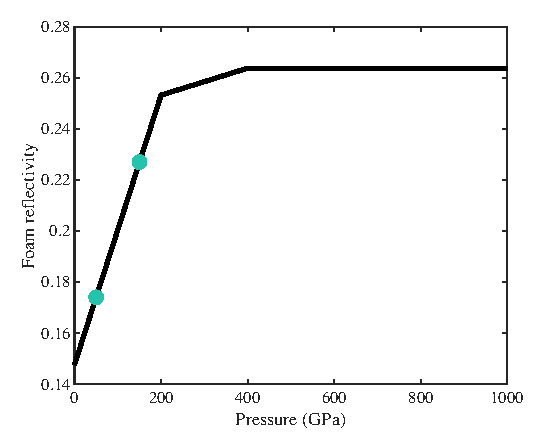
\includegraphics[width=0.6\textwidth]{figures/Experiment/FoamReflectivity.eps}% Here is how to import EPS art
\caption{\label{fig:Foam Reflectivity} The foam reflectivity model used in this work. The polystyrene pressure reflectivity model from \cite{Hu2014} has been scaled so that it passes through the two teal points; these were the results of two DFT simulations for the TMPTA material, performed for this experiment by collaborators at the University of Rochester. It can be seen that for the pressures of interest to this experiment, this is effectively just a linear relationship between the two points. However, this fit ensures that for any MC ransom samples at significantly higher pressures (statistically unlikely), the reflectivity will saturate rather than increasing indefinitely.}
\end{centering}
\end{figure}

As discussed in Section \ref{SOP theory}, the SOP setup was not absolutely calibrated and thus the calibration constant $A$ in Equation \ref{eqn: SOP eqn} could not be determined in advance, and the quartz was therefore used as an on-shot temperature reference. Equation \label{eqn:Temp fit} was used to estimate the expected quartz temperature, based on the the VISAR-determined shock velocity. This temperature and the maximum quartz SOP intensity from the SOP data were substituted into Equation \ref{eqn: SOP eqn} and used to determine $A$. This same calibration constant was then used for the foam data, and the maximum foam intensity was therefore used to calculate the foam shock temperature.

This approach has large uncertainties associated with it. The use of on-shot calibration means that the quartz temperature has to be estimated, based on the measured quartz shock velocity and fits to previous data; this will introduce error that will propagate through to the foam temperature. The models to estimate the quartz and foam uncertainty will also influence the final result. To capture all these contributors in the final uncertainty quantification, the same Monte Carlo analysis described in \ref{MC error} was applied. The same quartz shock velocity samples used for the impedance matching were also used to perform 10,000 iterations of the temperature calculation. As uncertainties for the various fits used were not quantified, estimates had to be made. The quartz temperature fit was assumed to have an uncertainty of 8\%, as this is the standard uncertainty for SOP temperature measurements at Omega \cite{Millot2015} (where the data for the fit was obtained). The quartz reflectivity fit was assumed to have a 10\% error, based on the size of the error bars in the published data \cite{Millot2015}. The foam reflectivity was given a large error of 0.1, to account for the uncertainty regarding this material (and lack of published experimental data). The streak counts for the quartz and foam measurements were assumed to be based on a Poisson distribution, with the uncertainty appropriate for that distribution used (the square root of the number of counts). The uncertainty in all these models were included in the MC analysis. As described in that section, the quoted temperature for each shot is the `exact' temperature (that obtained without sampling), while the error bars represent the standard deviation of the temperature distributions obtained using the MC methodology.

The results of the temperature measurements, compared to the theoretical modes, are displayed in FIGURE. These results will be discussed in SECTION.

\subsection{Comparing SOP timings to VISAR timings}
It was not possible to identify the breakout timings from each layer directly from the SOP data, as there was no clear change in signal corresponding to shock breakout from the quartz. However, the signal was expected to begin when the shock entered the quartz, and the foam signal was expected to peak at shock breakout from the foam. Based on this, it should be possible to determine a combined quartz/foam transit time that could be compared to the VISAR data.

The combined transit time for both the SOP and the VISAR data for all the valid experiment shots can be seen in Figure \ref{fig:SOP Timing}. The error bars on the SOP data are large; this is due to the large slit size used for the SOP (used to maximise signal strength), and the large sweep time. However, it can be seen that the agreement between the two diagnostics is good. This comparison serves two purposes. Firstly, it gives more confidence in the timing data for these two shots, as it is confirmed by two independent diagnostics. Secondly, it provides more confidence to the assumption that (despite the relatively low signal strength) the foam peak in the SOP data does in fact correspond to the foam breakout.

\begin{figure} [h!]
\begin{centering}
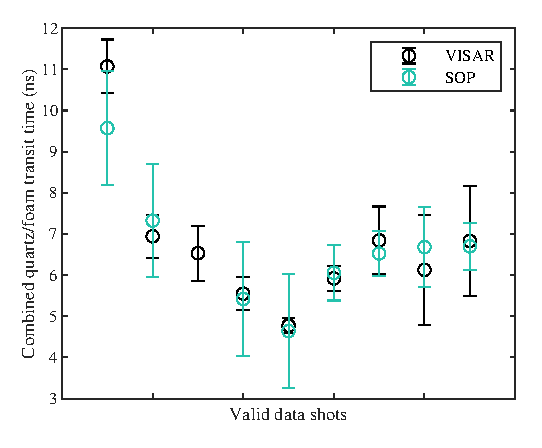
\includegraphics[width=0.6\textwidth]{figures/Experiment/SOPVISARtiming.eps}% Here is how to import EPS art
\caption{\label{fig:SOP Timing} The combined quartz/foam transit time measured using the VISAR (black) and SOP (teal).}
\end{centering}
\end{figure}

\subsection{Using the fiducial to estimate laser turn-on time}
As discussed in Section \ref{Fidu theory}, a fiducial on one of the VISAR streak cameras displayed the VULCAN pulse, and two-minute shots were performed to allow the time delay between the fiducial and the main pulse to be calculated. Three such shots were performed, and the data from one such shot is displayed. The time difference between the peak fiducial signal, and the peak of the (spatially-averaged) VULCAN signal, was calculated. This is shown for one of the two-minute shots in Figure \ref{fig:Two Minute}. This delay was averaged across the three shots to calculate the overall `fiducial delay'. 

\begin{figure} [h!]
\begin{centering}
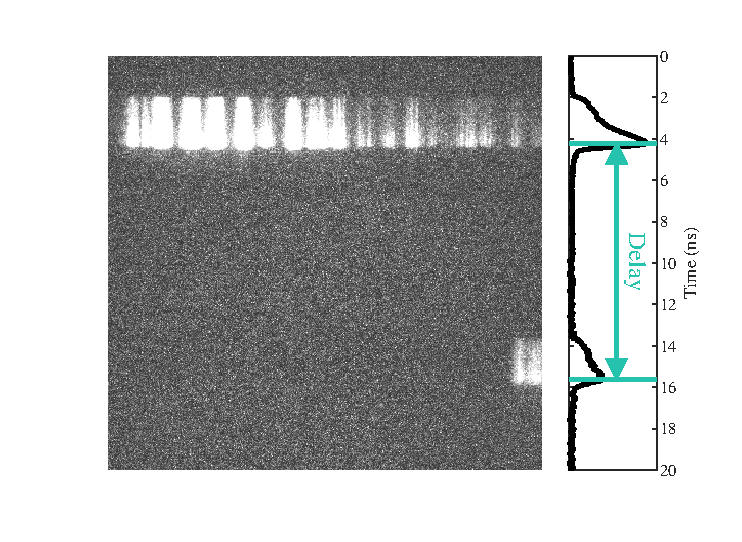
\includegraphics[width=0.7\textwidth]{figures/Experiment/TwoMinute.eps}% Here is how to import EPS art
\caption{\label{fig:Two Minute} VISAR streak for a two minute shot. The main VULCAN signal can be seen, along with the fiducial (on the bottom right of the image). On the right, a lineout is taken showing the average intensity of these signals (the fiducial is averaged only across the pixels where it appears, while the laser signal is averaged across the whole width of the image). The maximum intensity of each of these signals is identified (teal lines), and the delay time between them identified.}
\end{centering}
\end{figure}

The fiducial was not present for many of the early shots. For those where it was present the foot of the fiducial signal was identified, and the previously identified fiducial delay time was subtracted to find the time at which the VULCAN pulse was applied. This had an uncertainty associated with how accurately the fiducial delay could be calculated from the two minute shots, and how accurately the foot of the fiducial could be identified. If the quartz shock entry signal could be identified in the same VISAR streak as the fiducial, it was therefore possible to calculate the ablator/gold transit time - the time between when the laser was first applied and the quartz entry signal. This is shown in Figure \ref{fig:Fidu}. 

\begin{figure} [h]
\begin{centering}
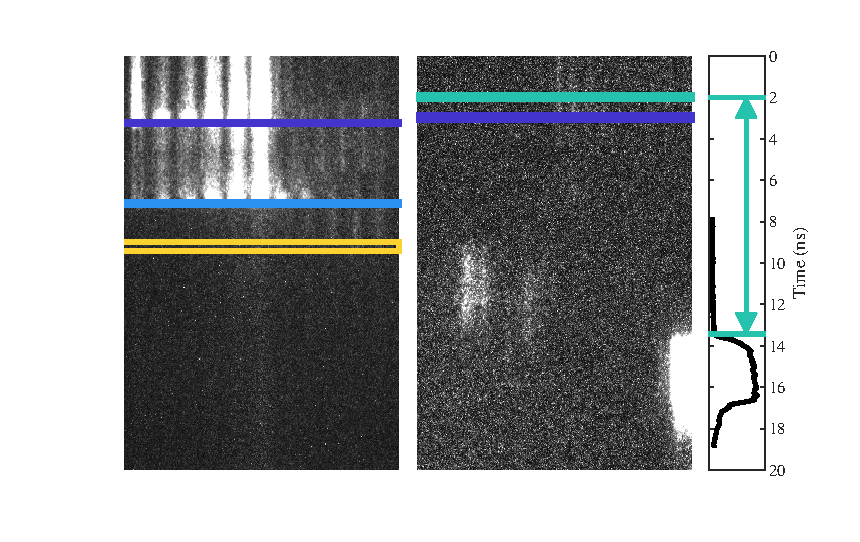
\includegraphics[width=0.9\textwidth]{figures/Experiment/FiduPlot.eps}% Here is how to import EPS art
\caption{\label{fig:Fidu} The two VISAR images for a shot where a fiducial was used. The fiducial is present on the second VISAR image. The trace on the right shows the intensity of the fiducial; it's start time is identified, and the delay time is used to estimate when the laser is first applied. This is plotted on the streak image (with uncertainty) in teal. The signal strength on this VISAR image is weak, and only the quartz entry signal (dark blue) is identified; this is sufficient to determine the abltor/gold transit time. The other signals (quartz breakout in light blue, foam breakout in orange) are identified from the other VISAR, where the signal strength is stronger. The data in this figure is for a different shot from the previous figures, as that shot did not have a working fiducial.}
\end{centering}
\end{figure}

\subsection{Estimating shot intensity}
The on-shot calorimetry provided a measure of the total VULCAN energy used on the shot. The phase plates were designed to produce a 400 \unit{\micro\meter} diameter, and the laser pulse time was reported by the laser team. These three pieces of information allowed the intensity to be quickly estimated. However, the additional diagnostics allowed the accuracy of this to be tested and improved.

The x-ray pinhole camera could be used to estimate the laser spot size. This diagnostic was not particularly accurate for such measurements, and was not intended to be used in the intensity calculation; but it could give a useful indication of whether the intended spot size was being achieved. An example pinhole camera image is displayed in Figure \ref{fig:Pinhole Analysis}.

\begin{figure} [h]
\begin{centering}
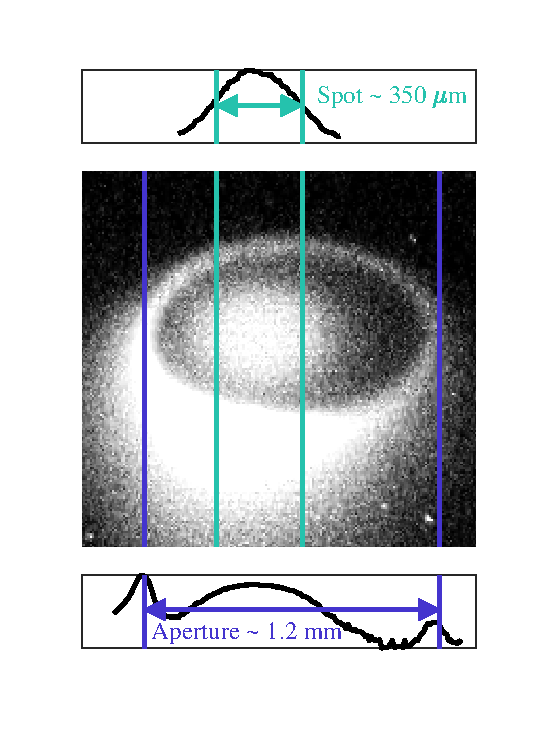
\includegraphics[width=0.6\textwidth]{figures/Experiment/PinholeAnalysis.eps}% Here is how to import EPS art
\caption{\label{fig:Pinhole Analysis} X-ray pinhole image for the standard data shot. A ring of emission is visible (corresponding to the copper shielding, with a known aperture of $\sim$ 1.2 \unit{\milli\meter} diameter, and the laser spot is visible in the middle of this. The trace below the image shows the log intensity of the signal over a narrow y-range, selected to capture the maximum diameter of the aperture. The position of peak signal either side of the aperture is identified (dark blue lines); this is assumed to be 1.2 \unit{\milli\meter}, providing a reference for the pixel scaling. The trace above the image shows the signal intensity over a narrow region corresponding to the maximum diameter position of the laser spot. The full width half maximum of the spot is then identified (teal lines); in this shot, this was found to be 350 \unit{\micro\meter}.}
\end{centering}
\end{figure}

The pinhole image showed a bright disk corresponding to the laser spot, with a bright halo corresponding to emission from the copper shielding. As the pinhole camera was positioned above the target the image is distorted in the y-direction, but the camera was normal to the target horizontally and thus the scaling in the x-direction is expected to be accurate. A narrow (in y) region was initially selected, positioned so that the aperture diameter was at it's maximum. The peak in emission either side of the aperture was identified. This can be seen on the trace below the image in Figure \ref{fig:Pinhole Analysis}. The distance between these peaks (i.e. the aperture diameter) was assumed to be equal to 1.2 \unit{\milli\meter}. Using this scaling, horizontal lengths could be calculated from number of pixels.

The trace above the image in Figure \ref{fig:Pinhole Analysis} shows the signal in another (narrow in y) region, corresponding to the peak horizontal diameter of the laser spot. The full-width half-maximum of this signal was then identified, and was measured (using the above scaling) as having a diameter of 350 \unit{\micro\meter}. This method is not expected to give a high accuracy for a variety of reasons (the laser spot clearly extends beyond the FWHM, the diameter of the aperture is assumed etc.), but this shows good agreement, suggesting that the phase plates are indeed resulting in a spot size of approximately 400 \unit{\micro\meter}. This was found to be the case for all the shots analysed in this way.

The laser pulse length could be determined using two methods. Firstly, the photodiode traces for each beam could be used. Traces were captured for each beam, but these could sometimes include noise/spurious signals, and were not accurately timed. Nonetheless, a reasonable estimate of the pulse length could be found by selecting the reasonable looking signals, shifting them to start at a similar time, and averaging them. This could then be compared to the requested pulse length, and normally showed very close agreement. On shots where the fiducial was present, it's intensity signal could also be used to estimate the temporal profile of the pulse. For both the traces and the fiducial, the full-width half-maximum was used as an estimate of the pulse length.

\begin{figure} [h]
\begin{centering}
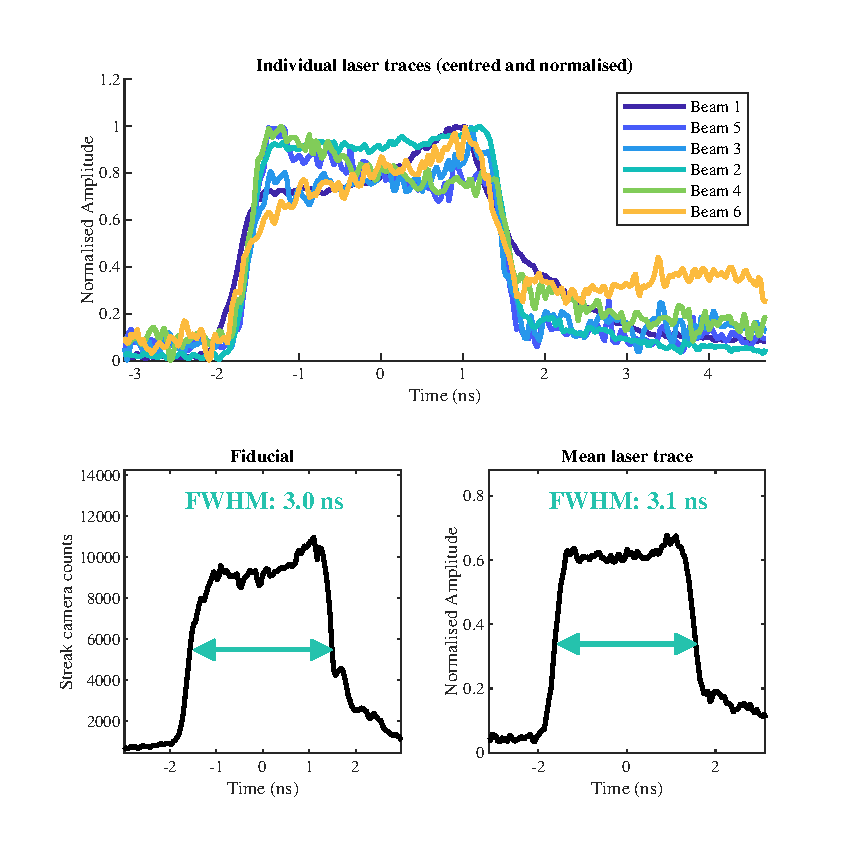
\includegraphics[width=0.8\textwidth]{figures/Experiment/FiduAndTrace.eps}% Here is how to import EPS art
\caption{\label{fig:Fidu and Trace} The laser pulse, as detected using the two methods, for shot 53. The top plot shows the individual traces for the 6 beams, each normalised and centred. The bottom right plot then averages these to approximate the overall pulse. The bottom left plot shows the intensity profile of the fiducial. The fiducial and average pulse can be seen to show good agreeement. The full width half maximum of either the fiducial or the combined traces can be used to approximate the pulse length.}
\end{centering}
\end{figure}

The laser energy was also calculated, using the on-shot calorimetry described in \hl{Section}. The laser intensity could therefore be estimated for each shot.

\subsection{Possible evidence of second shocks}

A small number of shots showed unexpected additional changes in signal in the VISAR and SOP data. The VISAR data would sometimes display a sudden increase in quartz signal strength part way through the quartz transit time. In the SOP, there would sometimes appear to be distinct periods of emission in the quartz. These two behaviours were often correlated. VISAR and SOP data for a shot where this is observed are displayed in Figure \ref{fig:Second Shock}.

\begin{figure} [h]
\begin{centering}
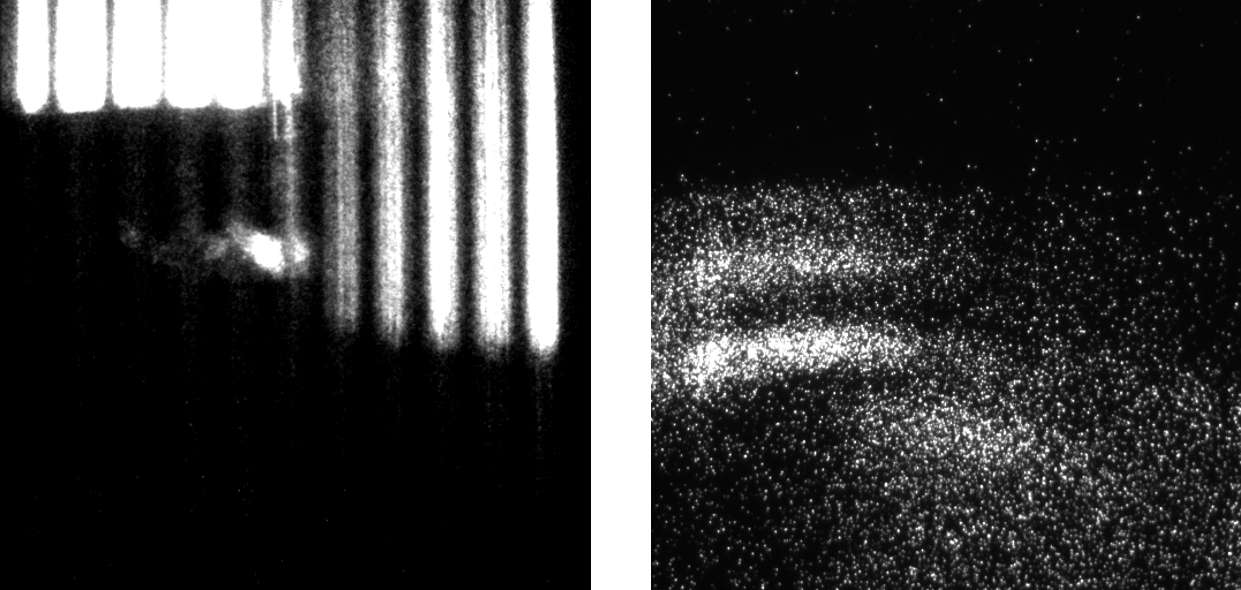
\includegraphics[width=1.0\textwidth]{figures/Experiment/Second Shock.png}% Here is how to import EPS art
\caption{\label{fig:Second Shock} VISAR (left) and SOP (right) data for a shot displaying a possible second shock. A sudden increase in the intensity of the VISAR signal is seen as the shock transits the quartz, which could correspond to a higher pressure shock with enhanced reflectivity. In the SOP signal, two distinct bands of emission within the quartz are observed.}
\end{centering}
\end{figure}

The most likely explanation for this would seem to be a second shock, which catches and overtakes the primary shock within the quartz layer. This would lead to a higher shock pressure being achieved in the quartz later in time (and thus an increased reflectivity and large VISAR signal), and an increase in shock temperature (and thus a region of second emission). Such a behaviour would mean that two shocks, of different velocity, contribute to the shock transit time - and thus the average velocity calculated from the VISAR data would not be physically meaningful. This would prevent an accurate impedance matching calculation from being performed. For this reason, any shots where such behaviour was observed were not included in the final results for this experiment.

The second shock phenomena was observed in the pre-hydrodynamic simulations for higher intensities, and is discussed in section \hl{section}. The increased quartz thickness used in the experiment (see Section \ref{Target issues}) also made this problem more likely, as did the higher intensities used (in order to try and generate stronger shocks). The post-shock simulations therefore suggested that the second shock could be an issue in this regime. However, this effect is difficult to simulate accurately. Post-shock simulations were performed of the shots for which the potential shock signals were observed, but the behaviour was not reproduced in simulations. This is a difficult phenomena to simulate - the state behind the first shock is already complicated, and will have some error/uncertainty compared to the real experimental conditions, and thus describing the transit of a second shock through this uncertain state is likely to have much larger uncertainty associated with it. In addition, later sections will demonstrate that there is a discrepancy between the shock strength in the quartz layer seen in the experiment relative to the simulations; such an effect would also impact any secondary shocks, leading to further uncertainty surrounding this effect. By omitting the shots where this behaviour is observed it is assumed that this effect has not had a significant impact on the experimental results; however, it is possible that in some shots the second shock would have undergone recombination in the foam, and this may not lead to an obvious signal.

\subsection{Intensity-shock strength relationship}

A plot of laser intensity vs the measured quartz and foam shock pressures is displayed in Figure \ref{fig:Intensity}. This plot provides a check on the data; it would be expected that the shock velocity would increase with laser intensity, and this in indeed seen to be the case. 

\begin{figure} [h]
\begin{centering}
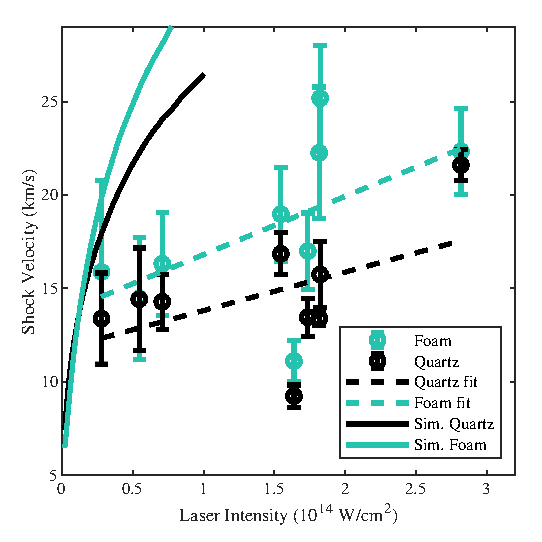
\includegraphics[width=0.6\textwidth]{figures/Experiment/Intensity.eps}% Here is how to import EPS art
\caption{\label{fig:Intensity} The measured shock velocity in the quartz (black) and foam (teal) as a function of intensity. The dashed lines show a linear fit to these two data sets, showing a general trend of increasing shock velocity with intensity. The solid lines show the results from pre-experiment 1D simulations.}
\end{centering}
\end{figure}

Secondly, the shock states achieved in the experiment were largely lower than expected, based on the pre-experiment hydrodynamic experiments. This plot demonstrates this to be the case - the lines show the simulated results, which occur at lower intensity. Interestingly, the curves appear to capture the trend of the data quite well, but are displaced to much lower intensities. This could suggest that the intensity achieved on each shot was actually significantly lower than expected; but based on the analysis in \hl{section}, this is unlikely to be the case. It could also be that the 1D and 2D hydrodynamic simulations overestiamted performance. While this likely is true, a discrepancy this large would not be expected. Finally, it could suggest that for some reason, the shock state for a given intensity is lower than expected for some additional, as yet undetermined reason. Later sections will demonstrate that this is believed to be the case.

\subsection{Analysis of glue targets and evidence for target delamination} \label{Glue targets}

As discussed in Section \ref{Target issues}, in some of the early targets the gold/CH coating delaminated from the quartz, and had to be glued back on. This resulted in a glue layer between the gold and quartz, which prevented the quartz transit time from being calculated - precluding any accurate measurements being made with these targets. Other than this glue layer, the targets were the same (although, as they were used as setup targets, they did not have a foam layer). However, as this occurred early on during setup, the targets were still shot (to save the better targets for later).

A disproportionate number of glue targets displayed fringe curvature. Of the glue targets that were shot and returned good signal strength, x/y displayed fringe motion. This was compared to x/y of the targets without a glue layer. As fringe motion required a minimum quartz pressure of 200 GPa, this suggested that the glued targets gave a greater chance of achieving higher shock strengths (and therefore shock pressures) in the quartz layer. In addition to this, a reference target consisting of a piece of stepped aluminium was also shot. In this target, the step was machined - meaning that the whole target was a single piece of aluminium, with no interface between targets. In this target it was possible to match the shock propagation times in a single simulation (although at a much lower intensity than was actually used in the experiment).

It was observed in \hl{Section} that the shock strength in the quartz appeared to be significantly weaker than in the Ch/gold layers. The glue target observations demonstrate that gluing these layers together reduces this difference, leading to a stronger quartz shock (although the glue prevents accurate shock timing measurements for the quartz, and thus it if the glue layer completely solves the discrepancy). This therefore suggests that poor contact between the glue and quartz layer is to blame for the reduced shock strength. This suggestion is also supported by the aluminium target, which suggested that without the interface this discrepancy is not observed. Given that full delamination was observed for some of the targets, it is suggested that partial delamination (resulting in gaps/voids between the layers, but not full separation) may have occurred in the other targets - resulting in a loss of shock strength as the shock crosses this interface.

\subsection{Trend between VISAR curvature and Pressure}

Prior to the experiment, it was expected that the quartz VISAR image would display fringe discontinuties and curvature, from which it would be possible to determine shock velocity. In fact this was rarely observed (and even when it was, the signal strength made actually calculating velocity from such signals infeasible. The most plausible explanation for this behaviour was that the quartz shock pressure was below the 200GPa required for the shock front to be reflective.

To test this assumption, a plot of quartz shock pressure (vs shock velocity) for the valid shots is included below. From this, there are two subtly conclusions that can be drawn. Firstly, most of the shots that displayed fringe discontinuities/curvature were above the required threshold (which provides additional confidence to the analysis and results, since this should be the case). Secondly, of the shots that achieved more than 200GPa, most did in fact display VISAR curvature. There are two exceptions to this - but by and large, the data fits the expecation. This therefore confirms that the reason for not observing this behaviour, rather than anything fundamentally wrong with the experiment, was that the achieved shock pressures were too low for the shock to be reflective.

\subsection{Simulation of a gap between layers}

Efforts were made to simulate the impact of a gap between these layers. Hyades simulations were performed using a low gas fill between the layers, or a Hyades `vacuum' zone - but this did not result in any reduction in shock strength in the quartz. Other simulations performed by our collaborators in Multi and Flash supported this.

However, it is possible that such an effect could not be captured in one-demensional hydrodynamics codes. Firstly, there is no obvious energy loss mechanism in 1D, and so once the gold material crosses the gap, the shock would continue undisturbed. This can also be demonstrated by the following simple model. When the shock reaches the rear target surface, it will undergo free surface expansion at roughly twice the shock velocity. If this is approximated as a plate flier at the shocked density (a very basic assumption, since in fact the expanding gold will have a strong density gradient), then the impact of the gold and quartz can be considered as a plate flier impedance match experiment. The solution to this interaction is a shock wave in the quartz with the exact same strength as if there had been no gap.

However, it is suggested that in a real interaction, there may be more losses. The shock will not be perfectly planar or uniform, and this will be exacerbated by the material crossing the gap. There could also be lateral energy transfer during this process. The process of shock-breakout is likely not perfectly clean and ideal, and all these factors could contribute to a reduction in the shock strength.

This was investigated in some 2D Flash simulations (these were performed by Piotr R\k{a}czka, although I suggested the target structure that should be used). Three dufferent gaps were simulated, with varying degrees of non-uniformity. It was observed that a non-uniform gap did appear to increase the shock transit time compared to a uniform one. Though this effect was small (and not sufficient to explain the experimental discrepancy), it does indicate that a non-uniform gap can lead to a loss of shock strength; particularly as in a real target, the gap is likely many times less uniform than that simulated here. 

\subsection{Shock stability}

\section{Final results}

\section{Comparison with other foam experiments}

\section{Suggested improvements}

